\documentclass[twoside]{book}

% Packages required by doxygen
\usepackage{fixltx2e}
\usepackage{calc}
\usepackage{doxygen}
\usepackage[export]{adjustbox} % also loads graphicx
\usepackage{graphicx}
\usepackage[utf8]{inputenc}
\usepackage{makeidx}
\usepackage{multicol}
\usepackage{multirow}
\PassOptionsToPackage{warn}{textcomp}
\usepackage{textcomp}
\usepackage[nointegrals]{wasysym}
\usepackage[table]{xcolor}

% Font selection
\usepackage[T1]{fontenc}
\usepackage[scaled=.90]{helvet}
\usepackage{courier}
\usepackage{amssymb}
\usepackage{sectsty}
\renewcommand{\familydefault}{\sfdefault}
\allsectionsfont{%
  \fontseries{bc}\selectfont%
  \color{darkgray}%
}
\renewcommand{\DoxyLabelFont}{%
  \fontseries{bc}\selectfont%
  \color{darkgray}%
}
\newcommand{\+}{\discretionary{\mbox{\scriptsize$\hookleftarrow$}}{}{}}

% Page & text layout
\usepackage{geometry}
\geometry{%
  a4paper,%
  top=2.5cm,%
  bottom=2.5cm,%
  left=2.5cm,%
  right=2.5cm%
}
\tolerance=750
\hfuzz=15pt
\hbadness=750
\setlength{\emergencystretch}{15pt}
\setlength{\parindent}{0cm}
\setlength{\parskip}{3ex plus 2ex minus 2ex}
\makeatletter
\renewcommand{\paragraph}{%
  \@startsection{paragraph}{4}{0ex}{-1.0ex}{1.0ex}{%
    \normalfont\normalsize\bfseries\SS@parafont%
  }%
}
\renewcommand{\subparagraph}{%
  \@startsection{subparagraph}{5}{0ex}{-1.0ex}{1.0ex}{%
    \normalfont\normalsize\bfseries\SS@subparafont%
  }%
}
\makeatother

% Headers & footers
\usepackage{fancyhdr}
\pagestyle{fancyplain}
\fancyhead[LE]{\fancyplain{}{\bfseries\thepage}}
\fancyhead[CE]{\fancyplain{}{}}
\fancyhead[RE]{\fancyplain{}{\bfseries\leftmark}}
\fancyhead[LO]{\fancyplain{}{\bfseries\rightmark}}
\fancyhead[CO]{\fancyplain{}{}}
\fancyhead[RO]{\fancyplain{}{\bfseries\thepage}}
\fancyfoot[LE]{\fancyplain{}{}}
\fancyfoot[CE]{\fancyplain{}{}}
\fancyfoot[RE]{\fancyplain{}{\bfseries\scriptsize Generated by Doxygen }}
\fancyfoot[LO]{\fancyplain{}{\bfseries\scriptsize Generated by Doxygen }}
\fancyfoot[CO]{\fancyplain{}{}}
\fancyfoot[RO]{\fancyplain{}{}}
\renewcommand{\footrulewidth}{0.4pt}
\renewcommand{\chaptermark}[1]{%
  \markboth{#1}{}%
}
\renewcommand{\sectionmark}[1]{%
  \markright{\thesection\ #1}%
}

% Indices & bibliography
\usepackage{natbib}
\usepackage[titles]{tocloft}
\setcounter{tocdepth}{3}
\setcounter{secnumdepth}{5}
\makeindex

% Hyperlinks (required, but should be loaded last)
\usepackage{ifpdf}
\ifpdf
  \usepackage[pdftex,pagebackref=true]{hyperref}
\else
  \usepackage[ps2pdf,pagebackref=true]{hyperref}
\fi
\hypersetup{%
  colorlinks=true,%
  linkcolor=blue,%
  citecolor=blue,%
  unicode%
}

% Custom commands
\newcommand{\clearemptydoublepage}{%
  \newpage{\pagestyle{empty}\cleardoublepage}%
}

\usepackage{caption}
\captionsetup{labelsep=space,justification=centering,font={bf},singlelinecheck=off,skip=4pt,position=top}

%===== C O N T E N T S =====

\begin{document}

% Titlepage & ToC
\hypersetup{pageanchor=false,
             bookmarksnumbered=true,
             pdfencoding=unicode
            }
\pagenumbering{alph}
\begin{titlepage}
\vspace*{7cm}
\begin{center}%
{\Large Atom \\[1ex]\large 1.\+0 }\\
\vspace*{1cm}
{\large Generated by Doxygen 1.8.13}\\
\end{center}
\end{titlepage}
\clearemptydoublepage
\pagenumbering{roman}
\tableofcontents
\clearemptydoublepage
\pagenumbering{arabic}
\hypersetup{pageanchor=true}

%--- Begin generated contents ---
\chapter{Main Page}
\label{index}\hypertarget{index}{}Implements a stack class

\begin{DoxyVersion}{Version}
4.\+0
\end{DoxyVersion}
\begin{DoxyAuthor}{Author}
ShJ 
\end{DoxyAuthor}
\begin{DoxyDate}{Date}
05.\+03.\+2017 
\end{DoxyDate}

\chapter{Namespace Index}
\section{Namespace List}
Here is a list of all documented namespaces with brief descriptions\+:\begin{DoxyCompactList}
\item\contentsline{section}{\hyperlink{namespaceatom}{atom} \\*Common namespace }{\pageref{namespaceatom}}{}
\end{DoxyCompactList}

\chapter{Hierarchical Index}
\section{Class Hierarchy}
This inheritance list is sorted roughly, but not completely, alphabetically\+:\begin{DoxyCompactList}
\item \contentsline{section}{atom\+:\+:array\+\_\+t$<$ Tp, max\+\_\+size\+\_\+ $>$}{\pageref{classatom_1_1array__t}}{}
\item \contentsline{section}{atom\+:\+:error}{\pageref{classatom_1_1error}}{}
\begin{DoxyCompactList}
\item \contentsline{section}{atom\+:\+:bad\+Alloc}{\pageref{classatom_1_1bad_alloc}}{}
\item \contentsline{section}{atom\+:\+:invalid\+Argument}{\pageref{classatom_1_1invalid_argument}}{}
\item \contentsline{section}{atom\+:\+:invalid\+Object}{\pageref{classatom_1_1invalid_object}}{}
\item \contentsline{section}{atom\+:\+:other\+Error}{\pageref{classatom_1_1other_error}}{}
\item \contentsline{section}{atom\+:\+:out\+Of\+Range}{\pageref{classatom_1_1out_of_range}}{}
\end{DoxyCompactList}
\item \contentsline{section}{P\+O\+I\+S\+ON$<$ Tp $>$}{\pageref{struct_p_o_i_s_o_n}}{}
\item \contentsline{section}{P\+O\+I\+S\+ON$<$ char $>$}{\pageref{struct_p_o_i_s_o_n_3_01char_01_4}}{}
\item \contentsline{section}{P\+O\+I\+S\+ON$<$ double $>$}{\pageref{struct_p_o_i_s_o_n_3_01double_01_4}}{}
\item \contentsline{section}{P\+O\+I\+S\+ON$<$ float $>$}{\pageref{struct_p_o_i_s_o_n_3_01float_01_4}}{}
\item \contentsline{section}{P\+O\+I\+S\+ON$<$ int $>$}{\pageref{struct_p_o_i_s_o_n_3_01int_01_4}}{}
\item \contentsline{section}{P\+O\+I\+S\+ON$<$ long long $>$}{\pageref{struct_p_o_i_s_o_n_3_01long_01long_01_4}}{}
\item \contentsline{section}{P\+O\+I\+S\+ON$<$ short $>$}{\pageref{struct_p_o_i_s_o_n_3_01short_01_4}}{}
\item \contentsline{section}{P\+O\+I\+S\+ON$<$ unsigned char $>$}{\pageref{struct_p_o_i_s_o_n_3_01unsigned_01char_01_4}}{}
\item \contentsline{section}{P\+O\+I\+S\+ON$<$ unsigned int $>$}{\pageref{struct_p_o_i_s_o_n_3_01unsigned_01int_01_4}}{}
\item \contentsline{section}{P\+O\+I\+S\+ON$<$ unsigned long long $>$}{\pageref{struct_p_o_i_s_o_n_3_01unsigned_01long_01long_01_4}}{}
\item \contentsline{section}{P\+O\+I\+S\+ON$<$ unsigned short $>$}{\pageref{struct_p_o_i_s_o_n_3_01unsigned_01short_01_4}}{}
\item \contentsline{section}{atom\+:\+:stack\+\_\+t$<$ Tp, Container $>$}{\pageref{classatom_1_1stack__t}}{}
\item \contentsline{section}{atom\+:\+:vector\+\_\+t$<$ Tp $>$}{\pageref{classatom_1_1vector__t}}{}
\end{DoxyCompactList}

\chapter{Class Index}
\section{Class List}
Here are the classes, structs, unions and interfaces with brief descriptions\+:\begin{DoxyCompactList}
\item\contentsline{section}{\hyperlink{classstk_1_1stack__t}{stk\+::stack\+\_\+t$<$ Tp $>$} }{\pageref{classstk_1_1stack__t}}{}
\end{DoxyCompactList}

\chapter{File Index}
\section{File List}
Here is a list of all documented files with brief descriptions\+:\begin{DoxyCompactList}
\item\contentsline{section}{D\+:/\+Git\+Hub/\+Techno\+Atom/src/\hyperlink{debug__tools_8h}{debug\+\_\+tools.\+h} }{\pageref{debug__tools_8h}}{}
\item\contentsline{section}{D\+:/\+Git\+Hub/\+Techno\+Atom/src/\hyperlink{exceptions_8h}{exceptions.\+h} }{\pageref{exceptions_8h}}{}
\item\contentsline{section}{D\+:/\+Git\+Hub/\+Techno\+Atom/src/array/\hyperlink{array_8h}{array.\+h} }{\pageref{array_8h}}{}
\item\contentsline{section}{D\+:/\+Git\+Hub/\+Techno\+Atom/src/array/implement/{\bfseries array.\+hpp} }{\pageref{array_8hpp}}{}
\item\contentsline{section}{D\+:/\+Git\+Hub/\+Techno\+Atom/src/stack/\hyperlink{stack_8h}{stack.\+h} }{\pageref{stack_8h}}{}
\item\contentsline{section}{D\+:/\+Git\+Hub/\+Techno\+Atom/src/stack/implement/{\bfseries stack.\+hpp} }{\pageref{stack_8hpp}}{}
\item\contentsline{section}{D\+:/\+Git\+Hub/\+Techno\+Atom/src/vector/\hyperlink{vector_8h}{vector.\+h} }{\pageref{vector_8h}}{}
\item\contentsline{section}{D\+:/\+Git\+Hub/\+Techno\+Atom/src/vector/implement/{\bfseries vector.\+hpp} }{\pageref{vector_8hpp}}{}
\end{DoxyCompactList}

\chapter{Namespace Documentation}
\hypertarget{namespaceatom}{}\section{atom Namespace Reference}
\label{namespaceatom}\index{atom@{atom}}


Common namespace.  


\subsection*{Classes}
\begin{DoxyCompactItemize}
\item 
class \hyperlink{classatom_1_1array__t}{array\+\_\+t}
\item 
class \hyperlink{classatom_1_1bad_alloc}{bad\+Alloc}
\begin{DoxyCompactList}\small\item\em Exception about problems with allocate of the memory. \end{DoxyCompactList}\item 
class \hyperlink{classatom_1_1error}{error}
\begin{DoxyCompactList}\small\item\em Abstract class which is template for all exceptions. \end{DoxyCompactList}\item 
class \hyperlink{classatom_1_1invalid_argument}{invalid\+Argument}
\begin{DoxyCompactList}\small\item\em Exception about problems with arguments in functions. \end{DoxyCompactList}\item 
class \hyperlink{classatom_1_1invalid_object}{invalid\+Object}
\begin{DoxyCompactList}\small\item\em Exception about problems with object different classes. \end{DoxyCompactList}\item 
class \hyperlink{classatom_1_1other_error}{other\+Error}
\begin{DoxyCompactList}\small\item\em Undefine here exceptions. \end{DoxyCompactList}\item 
class \hyperlink{classatom_1_1out_of_range}{out\+Of\+Range}
\begin{DoxyCompactList}\small\item\em Exception about problems connected with borders. \end{DoxyCompactList}\item 
class \hyperlink{classatom_1_1stack__t}{stack\+\_\+t}
\item 
class \hyperlink{classatom_1_1vector__t}{vector\+\_\+t}
\end{DoxyCompactItemize}


\subsection{Detailed Description}
Common namespace. 
\chapter{Class Documentation}
\hypertarget{classatom_1_1array__t}{}\section{atom\+:\+:array\+\_\+t$<$ Tp, max\+\_\+size\+\_\+ $>$ Class Template Reference}
\label{classatom_1_1array__t}\index{atom\+::array\+\_\+t$<$ Tp, max\+\_\+size\+\_\+ $>$@{atom\+::array\+\_\+t$<$ Tp, max\+\_\+size\+\_\+ $>$}}


{\ttfamily \#include $<$array.\+h$>$}



Collaboration diagram for atom\+:\+:array\+\_\+t$<$ Tp, max\+\_\+size\+\_\+ $>$\+:
\nopagebreak
\begin{figure}[H]
\begin{center}
\leavevmode
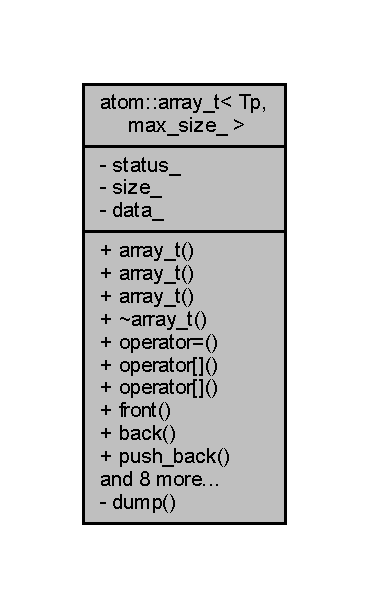
\includegraphics[width=177pt]{classatom_1_1array__t__coll__graph}
\end{center}
\end{figure}
\subsection*{Public Types}
\begin{DoxyCompactItemize}
\item 
\mbox{\Hypertarget{classatom_1_1array__t_aeb485cd6190dc11ddb8e7f48c09451c4}\label{classatom_1_1array__t_aeb485cd6190dc11ddb8e7f48c09451c4}} 
using \hyperlink{classatom_1_1array__t_aeb485cd6190dc11ddb8e7f48c09451c4}{value\+\_\+type} = Tp
\begin{DoxyCompactList}\small\item\em Element type. \end{DoxyCompactList}\item 
\mbox{\Hypertarget{classatom_1_1array__t_a9c33ee3fb4e5b4d57c7801a8f69ada14}\label{classatom_1_1array__t_a9c33ee3fb4e5b4d57c7801a8f69ada14}} 
using \hyperlink{classatom_1_1array__t_a9c33ee3fb4e5b4d57c7801a8f69ada14}{const\+\_\+value\+\_\+type} = const Tp
\begin{DoxyCompactList}\small\item\em Const element type. \end{DoxyCompactList}\item 
\mbox{\Hypertarget{classatom_1_1array__t_a8534f23c7f0082698cbd708e1f2e26ff}\label{classatom_1_1array__t_a8534f23c7f0082698cbd708e1f2e26ff}} 
using \hyperlink{classatom_1_1array__t_a8534f23c7f0082698cbd708e1f2e26ff}{size\+\_\+type} = std\+::size\+\_\+t
\begin{DoxyCompactList}\small\item\em Size type. \end{DoxyCompactList}\end{DoxyCompactItemize}
\subsection*{Public Member Functions}
\begin{DoxyCompactItemize}
\item 
\hyperlink{classatom_1_1array__t_ac909dffe60e64d871a3c23e74480cdf1}{array\+\_\+t} () noexcept
\begin{DoxyCompactList}\small\item\em Default constructor. \end{DoxyCompactList}\item 
\hyperlink{classatom_1_1array__t_a9f3f72a3c77e55f6f18bfcfb065b78b3}{array\+\_\+t} (const \hyperlink{classatom_1_1array__t_a8534f23c7f0082698cbd708e1f2e26ff}{size\+\_\+type} n, const \hyperlink{classatom_1_1array__t_aeb485cd6190dc11ddb8e7f48c09451c4}{value\+\_\+type} \&value=\hyperlink{classatom_1_1array__t_aeb485cd6190dc11ddb8e7f48c09451c4}{value\+\_\+type}())
\begin{DoxyCompactList}\small\item\em Constructor. \end{DoxyCompactList}\item 
\mbox{\Hypertarget{classatom_1_1array__t_a90c35f817089cdefbfc68a493dac97cf}\label{classatom_1_1array__t_a90c35f817089cdefbfc68a493dac97cf}} 
\hyperlink{classatom_1_1array__t_a90c35f817089cdefbfc68a493dac97cf}{array\+\_\+t} (const \hyperlink{classatom_1_1array__t}{array\+\_\+t} \&that)=default
\begin{DoxyCompactList}\small\item\em Default copy constructor. \end{DoxyCompactList}\item 
\hyperlink{classatom_1_1array__t_afc5abfb4d2764ef27b0fb237e4dd63a3}{$\sim$array\+\_\+t} ()
\begin{DoxyCompactList}\small\item\em Default destructor. \end{DoxyCompactList}\item 
const \hyperlink{classatom_1_1array__t}{array\+\_\+t} \& \hyperlink{classatom_1_1array__t_aee988e07623e2c643765a286eb52eea6}{operator=} (const \hyperlink{classatom_1_1array__t}{array\+\_\+t} \&that)
\begin{DoxyCompactList}\small\item\em The assignment operator. \end{DoxyCompactList}\item 
\hyperlink{classatom_1_1array__t_a9c33ee3fb4e5b4d57c7801a8f69ada14}{const\+\_\+value\+\_\+type} \& \hyperlink{classatom_1_1array__t_aa6995427dae0b4a3ce63d8fd47ed3121}{operator\mbox{[}$\,$\mbox{]}} (const \hyperlink{classatom_1_1array__t_a8534f23c7f0082698cbd708e1f2e26ff}{size\+\_\+type} n) const
\begin{DoxyCompactList}\small\item\em Operator addressing. \end{DoxyCompactList}\item 
\hyperlink{classatom_1_1array__t_aeb485cd6190dc11ddb8e7f48c09451c4}{value\+\_\+type} \& \hyperlink{classatom_1_1array__t_ad96738ee0018dce88aaeb9941c24dee0}{operator\mbox{[}$\,$\mbox{]}} (const \hyperlink{classatom_1_1array__t_a8534f23c7f0082698cbd708e1f2e26ff}{size\+\_\+type} n)
\begin{DoxyCompactList}\small\item\em Operator addressing. \end{DoxyCompactList}\item 
\hyperlink{classatom_1_1array__t_a9c33ee3fb4e5b4d57c7801a8f69ada14}{const\+\_\+value\+\_\+type} \& \hyperlink{classatom_1_1array__t_a3ef0f195a147615aa53a3e2a47c61c49}{front} () const
\begin{DoxyCompactList}\small\item\em First element. \end{DoxyCompactList}\item 
\hyperlink{classatom_1_1array__t_a9c33ee3fb4e5b4d57c7801a8f69ada14}{const\+\_\+value\+\_\+type} \& \hyperlink{classatom_1_1array__t_a2337c7353a06e7df164112021138f7fd}{back} () const
\begin{DoxyCompactList}\small\item\em Last element. \end{DoxyCompactList}\item 
void \hyperlink{classatom_1_1array__t_ad53d9e0a290e125927d70c202b04aea4}{push\+\_\+back} (\hyperlink{classatom_1_1array__t_a9c33ee3fb4e5b4d57c7801a8f69ada14}{const\+\_\+value\+\_\+type} x)
\begin{DoxyCompactList}\small\item\em Push new item in back of the array. \end{DoxyCompactList}\item 
bool \hyperlink{classatom_1_1array__t_a2d07b56eadfc3c1aed378d918366f859}{erase} (const \hyperlink{classatom_1_1array__t_a8534f23c7f0082698cbd708e1f2e26ff}{size\+\_\+type} position)
\begin{DoxyCompactList}\small\item\em Remove nth element. \end{DoxyCompactList}\item 
bool \hyperlink{classatom_1_1array__t_aac24cc1d7dab76ac0bf394aaa8699e27}{empty} () const noexcept
\begin{DoxyCompactList}\small\item\em Checks the array on the void. \end{DoxyCompactList}\item 
\hyperlink{classatom_1_1array__t_a8534f23c7f0082698cbd708e1f2e26ff}{size\+\_\+type} \hyperlink{classatom_1_1array__t_ab399c935e3103360bcd3aacd79d3bd06}{size} () const noexcept
\begin{DoxyCompactList}\small\item\em Size. \end{DoxyCompactList}\item 
\hyperlink{classatom_1_1array__t_a8534f23c7f0082698cbd708e1f2e26ff}{size\+\_\+type} \hyperlink{classatom_1_1array__t_a83235683c8ca9bceb07d050ae1efe767}{capacity} () const noexcept
\begin{DoxyCompactList}\small\item\em Capacity. \end{DoxyCompactList}\item 
void \hyperlink{classatom_1_1array__t_a3062d6888dd690495402b2dadbafe727}{fill} (\hyperlink{classatom_1_1array__t_a9c33ee3fb4e5b4d57c7801a8f69ada14}{const\+\_\+value\+\_\+type} \&value)
\begin{DoxyCompactList}\small\item\em Fill the array. \end{DoxyCompactList}\item 
bool \hyperlink{classatom_1_1array__t_a44737f61d6cac6e2a65fbee06b702755}{use\+\_\+array} (const \hyperlink{classatom_1_1array__t_a8534f23c7f0082698cbd708e1f2e26ff}{size\+\_\+type} n) noexcept
\begin{DoxyCompactList}\small\item\em Set new size of the array within max\+\_\+size. \end{DoxyCompactList}\item 
void \hyperlink{classatom_1_1array__t_a139e38b7e830dc58885a768fe135dee5}{swap} (\hyperlink{classatom_1_1array__t}{array\+\_\+t} \&rhs)
\begin{DoxyCompactList}\small\item\em Swap two array. \end{DoxyCompactList}\item 
bool \hyperlink{classatom_1_1array__t_a6a069628b26cc592466475ec97ff362a}{is\+\_\+valid} () const noexcept
\begin{DoxyCompactList}\small\item\em Silent verifier. \end{DoxyCompactList}\end{DoxyCompactItemize}
\subsection*{Private Member Functions}
\begin{DoxyCompactItemize}
\item 
void \hyperlink{classatom_1_1array__t_a3e133e59958e8638b0f6d7a74b9890d6}{dump} (const char $\ast$function\+\_\+name, int line\+\_\+number) const
\begin{DoxyCompactList}\small\item\em Dumper. \end{DoxyCompactList}\end{DoxyCompactItemize}
\subsection*{Private Attributes}
\begin{DoxyCompactItemize}
\item 
\mbox{\Hypertarget{classatom_1_1array__t_a621a080eeb6d2d7501221fed64f3a1d1}\label{classatom_1_1array__t_a621a080eeb6d2d7501221fed64f3a1d1}} 
bool \hyperlink{classatom_1_1array__t_a621a080eeb6d2d7501221fed64f3a1d1}{status\+\_\+}
\begin{DoxyCompactList}\small\item\em Status of the array. \end{DoxyCompactList}\item 
\mbox{\Hypertarget{classatom_1_1array__t_a56208ec116be4941be22dde2f921203e}\label{classatom_1_1array__t_a56208ec116be4941be22dde2f921203e}} 
\hyperlink{classatom_1_1array__t_a8534f23c7f0082698cbd708e1f2e26ff}{size\+\_\+type} \hyperlink{classatom_1_1array__t_a56208ec116be4941be22dde2f921203e}{size\+\_\+}
\begin{DoxyCompactList}\small\item\em Size of the array. \end{DoxyCompactList}\item 
\mbox{\Hypertarget{classatom_1_1array__t_afb74074f5cc1bb0dc10c6c556ecb12d4}\label{classatom_1_1array__t_afb74074f5cc1bb0dc10c6c556ecb12d4}} 
\hyperlink{classatom_1_1array__t_aeb485cd6190dc11ddb8e7f48c09451c4}{value\+\_\+type} \hyperlink{classatom_1_1array__t_afb74074f5cc1bb0dc10c6c556ecb12d4}{data\+\_\+} \mbox{[}max\+\_\+size\+\_\+\mbox{]}
\begin{DoxyCompactList}\small\item\em Buffer of the array. \end{DoxyCompactList}\end{DoxyCompactItemize}


\subsection{Detailed Description}
\subsubsection*{template$<$typename Tp, const std\+::size\+\_\+t max\+\_\+size\+\_\+ = 256$>$\newline
class atom\+::array\+\_\+t$<$ Tp, max\+\_\+size\+\_\+ $>$}


\begin{DoxyTemplParams}{Template Parameters}
{\em Tp} & The type of the value in the array \\
\hline
{\em max\+\_\+size\+\_\+} & Max capacity of the array (default is 256) \\
\hline
\end{DoxyTemplParams}


\subsection{Constructor \& Destructor Documentation}
\mbox{\Hypertarget{classatom_1_1array__t_ac909dffe60e64d871a3c23e74480cdf1}\label{classatom_1_1array__t_ac909dffe60e64d871a3c23e74480cdf1}} 
\index{atom\+::array\+\_\+t@{atom\+::array\+\_\+t}!array\+\_\+t@{array\+\_\+t}}
\index{array\+\_\+t@{array\+\_\+t}!atom\+::array\+\_\+t@{atom\+::array\+\_\+t}}
\subsubsection{\texorpdfstring{array\+\_\+t()}{array\_t()}\hspace{0.1cm}{\footnotesize\ttfamily [1/2]}}
{\footnotesize\ttfamily template$<$typename Tp, const std\+::size\+\_\+t max\+\_\+size\+\_\+ = 256$>$ \\
\hyperlink{classatom_1_1array__t}{atom\+::array\+\_\+t}$<$ Tp, max\+\_\+size\+\_\+ $>$\+::\hyperlink{classatom_1_1array__t}{array\+\_\+t} (\begin{DoxyParamCaption}{ }\end{DoxyParamCaption})\hspace{0.3cm}{\ttfamily [inline]}, {\ttfamily [noexcept]}}



Default constructor. 

When switched debug fill all elements of the \hyperlink{struct_p_o_i_s_o_n}{P\+O\+I\+S\+ON} \mbox{\Hypertarget{classatom_1_1array__t_a9f3f72a3c77e55f6f18bfcfb065b78b3}\label{classatom_1_1array__t_a9f3f72a3c77e55f6f18bfcfb065b78b3}} 
\index{atom\+::array\+\_\+t@{atom\+::array\+\_\+t}!array\+\_\+t@{array\+\_\+t}}
\index{array\+\_\+t@{array\+\_\+t}!atom\+::array\+\_\+t@{atom\+::array\+\_\+t}}
\subsubsection{\texorpdfstring{array\+\_\+t()}{array\_t()}\hspace{0.1cm}{\footnotesize\ttfamily [2/2]}}
{\footnotesize\ttfamily template$<$typename Tp, const std\+::size\+\_\+t max\+\_\+size\+\_\+ = 256$>$ \\
\hyperlink{classatom_1_1array__t}{atom\+::array\+\_\+t}$<$ Tp, max\+\_\+size\+\_\+ $>$\+::\hyperlink{classatom_1_1array__t}{array\+\_\+t} (\begin{DoxyParamCaption}\item[{const \hyperlink{classatom_1_1array__t_a8534f23c7f0082698cbd708e1f2e26ff}{size\+\_\+type}}]{n,  }\item[{const \hyperlink{classatom_1_1array__t_aeb485cd6190dc11ddb8e7f48c09451c4}{value\+\_\+type} \&}]{value = {\ttfamily \hyperlink{classatom_1_1array__t_aeb485cd6190dc11ddb8e7f48c09451c4}{value\+\_\+type}()} }\end{DoxyParamCaption})\hspace{0.3cm}{\ttfamily [inline]}}



Constructor. 

Constructor which set size of the array and initialize them

Macro A\+T\+O\+M\+\_\+\+N\+D\+E\+B\+UG for debug mode 
\begin{DoxyParams}{Parameters}
{\em n} & The desired size of the array \\
\hline
{\em value} & (default \hyperlink{classatom_1_1array__t_aeb485cd6190dc11ddb8e7f48c09451c4}{value\+\_\+type()}) initializer for n elements \\
\hline
\end{DoxyParams}

\begin{DoxyExceptions}{Exceptions}
{\em \hyperlink{classatom_1_1bad_alloc}{atom\+::bad\+Alloc}} & If n less than max size \\
\hline
\end{DoxyExceptions}
\mbox{\Hypertarget{classatom_1_1array__t_afc5abfb4d2764ef27b0fb237e4dd63a3}\label{classatom_1_1array__t_afc5abfb4d2764ef27b0fb237e4dd63a3}} 
\index{atom\+::array\+\_\+t@{atom\+::array\+\_\+t}!````~array\+\_\+t@{$\sim$array\+\_\+t}}
\index{````~array\+\_\+t@{$\sim$array\+\_\+t}!atom\+::array\+\_\+t@{atom\+::array\+\_\+t}}
\subsubsection{\texorpdfstring{$\sim$array\+\_\+t()}{~array\_t()}}
{\footnotesize\ttfamily template$<$typename Tp, const std\+::size\+\_\+t max\+\_\+size\+\_\+ = 256$>$ \\
\hyperlink{classatom_1_1array__t}{atom\+::array\+\_\+t}$<$ Tp, max\+\_\+size\+\_\+ $>$\+::$\sim$\hyperlink{classatom_1_1array__t}{array\+\_\+t} (\begin{DoxyParamCaption}{ }\end{DoxyParamCaption})\hspace{0.3cm}{\ttfamily [inline]}}



Default destructor. 

Macro A\+T\+O\+M\+\_\+\+N\+D\+E\+B\+UG for debug mode 

\subsection{Member Function Documentation}
\mbox{\Hypertarget{classatom_1_1array__t_a2337c7353a06e7df164112021138f7fd}\label{classatom_1_1array__t_a2337c7353a06e7df164112021138f7fd}} 
\index{atom\+::array\+\_\+t@{atom\+::array\+\_\+t}!back@{back}}
\index{back@{back}!atom\+::array\+\_\+t@{atom\+::array\+\_\+t}}
\subsubsection{\texorpdfstring{back()}{back()}}
{\footnotesize\ttfamily template$<$typename Tp, const std\+::size\+\_\+t max\+\_\+size\+\_\+ = 256$>$ \\
\hyperlink{classatom_1_1array__t_a9c33ee3fb4e5b4d57c7801a8f69ada14}{const\+\_\+value\+\_\+type}\& \hyperlink{classatom_1_1array__t}{atom\+::array\+\_\+t}$<$ Tp, max\+\_\+size\+\_\+ $>$\+::back (\begin{DoxyParamCaption}{ }\end{DoxyParamCaption}) const\hspace{0.3cm}{\ttfamily [inline]}}



Last element. 


\begin{DoxyExceptions}{Exceptions}
{\em The} & same exceptions as the operator\mbox{[}\mbox{]} \\
\hline
\end{DoxyExceptions}
\mbox{\Hypertarget{classatom_1_1array__t_a83235683c8ca9bceb07d050ae1efe767}\label{classatom_1_1array__t_a83235683c8ca9bceb07d050ae1efe767}} 
\index{atom\+::array\+\_\+t@{atom\+::array\+\_\+t}!capacity@{capacity}}
\index{capacity@{capacity}!atom\+::array\+\_\+t@{atom\+::array\+\_\+t}}
\subsubsection{\texorpdfstring{capacity()}{capacity()}}
{\footnotesize\ttfamily template$<$typename Tp, const std\+::size\+\_\+t max\+\_\+size\+\_\+ = 256$>$ \\
\hyperlink{classatom_1_1array__t_a8534f23c7f0082698cbd708e1f2e26ff}{size\+\_\+type} \hyperlink{classatom_1_1array__t}{atom\+::array\+\_\+t}$<$ Tp, max\+\_\+size\+\_\+ $>$\+::capacity (\begin{DoxyParamCaption}{ }\end{DoxyParamCaption}) const\hspace{0.3cm}{\ttfamily [inline]}, {\ttfamily [noexcept]}}



Capacity. 

\begin{DoxyReturn}{Returns}
capacity of the array 
\end{DoxyReturn}
\mbox{\Hypertarget{classatom_1_1array__t_a3e133e59958e8638b0f6d7a74b9890d6}\label{classatom_1_1array__t_a3e133e59958e8638b0f6d7a74b9890d6}} 
\index{atom\+::array\+\_\+t@{atom\+::array\+\_\+t}!dump@{dump}}
\index{dump@{dump}!atom\+::array\+\_\+t@{atom\+::array\+\_\+t}}
\subsubsection{\texorpdfstring{dump()}{dump()}}
{\footnotesize\ttfamily template$<$typename Tp , std\+::size\+\_\+t max\+\_\+size\+\_\+$>$ \\
void \hyperlink{classatom_1_1array__t}{atom\+::array\+\_\+t}$<$ Tp, max\+\_\+size\+\_\+ $>$\+::dump (\begin{DoxyParamCaption}\item[{const char $\ast$}]{function\+\_\+name,  }\item[{int}]{line\+\_\+number }\end{DoxyParamCaption}) const\hspace{0.3cm}{\ttfamily [private]}}



Dumper. 

Create file \char`\"{}\+\_\+\+\_\+array\+\_\+dump.\+txt\char`\"{} where is information about array\textquotesingle{}s status

Macro A\+T\+O\+M\+\_\+\+N\+W\+R\+I\+TE prohibit function \hyperlink{classatom_1_1array__t_a3e133e59958e8638b0f6d7a74b9890d6}{dump()} print elements (for example when value\+\_\+type has not operator$<$$<$) 
\begin{DoxyParams}{Parameters}
{\em function\+\_\+name} & Name of function which call this method \\
\hline
{\em line\+\_\+number} & Number of line which call this method \\
\hline
\end{DoxyParams}
\mbox{\Hypertarget{classatom_1_1array__t_aac24cc1d7dab76ac0bf394aaa8699e27}\label{classatom_1_1array__t_aac24cc1d7dab76ac0bf394aaa8699e27}} 
\index{atom\+::array\+\_\+t@{atom\+::array\+\_\+t}!empty@{empty}}
\index{empty@{empty}!atom\+::array\+\_\+t@{atom\+::array\+\_\+t}}
\subsubsection{\texorpdfstring{empty()}{empty()}}
{\footnotesize\ttfamily template$<$typename Tp, const std\+::size\+\_\+t max\+\_\+size\+\_\+ = 256$>$ \\
bool \hyperlink{classatom_1_1array__t}{atom\+::array\+\_\+t}$<$ Tp, max\+\_\+size\+\_\+ $>$\+::empty (\begin{DoxyParamCaption}{ }\end{DoxyParamCaption}) const\hspace{0.3cm}{\ttfamily [inline]}, {\ttfamily [noexcept]}}



Checks the array on the void. 

\begin{DoxyReturn}{Returns}
True if array is empty, otherwise false 
\end{DoxyReturn}
\mbox{\Hypertarget{classatom_1_1array__t_a2d07b56eadfc3c1aed378d918366f859}\label{classatom_1_1array__t_a2d07b56eadfc3c1aed378d918366f859}} 
\index{atom\+::array\+\_\+t@{atom\+::array\+\_\+t}!erase@{erase}}
\index{erase@{erase}!atom\+::array\+\_\+t@{atom\+::array\+\_\+t}}
\subsubsection{\texorpdfstring{erase()}{erase()}}
{\footnotesize\ttfamily template$<$typename Tp, const std\+::size\+\_\+t max\+\_\+size\+\_\+ = 256$>$ \\
bool \hyperlink{classatom_1_1array__t}{atom\+::array\+\_\+t}$<$ Tp, max\+\_\+size\+\_\+ $>$\+::erase (\begin{DoxyParamCaption}\item[{const \hyperlink{classatom_1_1array__t_a8534f23c7f0082698cbd708e1f2e26ff}{size\+\_\+type}}]{position }\end{DoxyParamCaption})\hspace{0.3cm}{\ttfamily [inline]}}



Remove nth element. 

Macro A\+T\+O\+M\+\_\+\+N\+D\+E\+B\+UG for debug mode 
\begin{DoxyParams}{Parameters}
{\em position} & number of the item in the array \\
\hline
\end{DoxyParams}

\begin{DoxyExceptions}{Exceptions}
{\em \hyperlink{classatom_1_1invalid_object}{atom\+::invalid\+Object}} & From \hyperlink{debug__tools_8h_a273b49426c51bc6a7eb989ee0acbdc6b}{A\+T\+O\+M\+\_\+\+A\+S\+S\+E\+R\+T\+\_\+\+V\+A\+L\+I\+D()} when array is not valid \\
\hline
\end{DoxyExceptions}
\begin{DoxyReturn}{Returns}
True if element was delete, otherwise false 
\end{DoxyReturn}
\mbox{\Hypertarget{classatom_1_1array__t_a3062d6888dd690495402b2dadbafe727}\label{classatom_1_1array__t_a3062d6888dd690495402b2dadbafe727}} 
\index{atom\+::array\+\_\+t@{atom\+::array\+\_\+t}!fill@{fill}}
\index{fill@{fill}!atom\+::array\+\_\+t@{atom\+::array\+\_\+t}}
\subsubsection{\texorpdfstring{fill()}{fill()}}
{\footnotesize\ttfamily template$<$typename Tp, const std\+::size\+\_\+t max\+\_\+size\+\_\+ = 256$>$ \\
void \hyperlink{classatom_1_1array__t}{atom\+::array\+\_\+t}$<$ Tp, max\+\_\+size\+\_\+ $>$\+::fill (\begin{DoxyParamCaption}\item[{\hyperlink{classatom_1_1array__t_a9c33ee3fb4e5b4d57c7801a8f69ada14}{const\+\_\+value\+\_\+type} \&}]{value }\end{DoxyParamCaption})\hspace{0.3cm}{\ttfamily [inline]}}



Fill the array. 


\begin{DoxyParams}{Parameters}
{\em value} & The value to be assigned to all elements of the array \\
\hline
\end{DoxyParams}
\mbox{\Hypertarget{classatom_1_1array__t_a3ef0f195a147615aa53a3e2a47c61c49}\label{classatom_1_1array__t_a3ef0f195a147615aa53a3e2a47c61c49}} 
\index{atom\+::array\+\_\+t@{atom\+::array\+\_\+t}!front@{front}}
\index{front@{front}!atom\+::array\+\_\+t@{atom\+::array\+\_\+t}}
\subsubsection{\texorpdfstring{front()}{front()}}
{\footnotesize\ttfamily template$<$typename Tp, const std\+::size\+\_\+t max\+\_\+size\+\_\+ = 256$>$ \\
\hyperlink{classatom_1_1array__t_a9c33ee3fb4e5b4d57c7801a8f69ada14}{const\+\_\+value\+\_\+type}\& \hyperlink{classatom_1_1array__t}{atom\+::array\+\_\+t}$<$ Tp, max\+\_\+size\+\_\+ $>$\+::front (\begin{DoxyParamCaption}{ }\end{DoxyParamCaption}) const\hspace{0.3cm}{\ttfamily [inline]}}



First element. 


\begin{DoxyExceptions}{Exceptions}
{\em The} & same exceptions as the operator\mbox{[}\mbox{]} \\
\hline
\end{DoxyExceptions}
\mbox{\Hypertarget{classatom_1_1array__t_a6a069628b26cc592466475ec97ff362a}\label{classatom_1_1array__t_a6a069628b26cc592466475ec97ff362a}} 
\index{atom\+::array\+\_\+t@{atom\+::array\+\_\+t}!is\+\_\+valid@{is\+\_\+valid}}
\index{is\+\_\+valid@{is\+\_\+valid}!atom\+::array\+\_\+t@{atom\+::array\+\_\+t}}
\subsubsection{\texorpdfstring{is\+\_\+valid()}{is\_valid()}}
{\footnotesize\ttfamily template$<$typename Tp, const std\+::size\+\_\+t max\+\_\+size\+\_\+ = 256$>$ \\
bool \hyperlink{classatom_1_1array__t}{atom\+::array\+\_\+t}$<$ Tp, max\+\_\+size\+\_\+ $>$\+::is\+\_\+valid (\begin{DoxyParamCaption}{ }\end{DoxyParamCaption}) const\hspace{0.3cm}{\ttfamily [inline]}, {\ttfamily [noexcept]}}



Silent verifier. 

\begin{DoxyReturn}{Returns}
True if array is valid else return false 
\end{DoxyReturn}
\mbox{\Hypertarget{classatom_1_1array__t_aee988e07623e2c643765a286eb52eea6}\label{classatom_1_1array__t_aee988e07623e2c643765a286eb52eea6}} 
\index{atom\+::array\+\_\+t@{atom\+::array\+\_\+t}!operator=@{operator=}}
\index{operator=@{operator=}!atom\+::array\+\_\+t@{atom\+::array\+\_\+t}}
\subsubsection{\texorpdfstring{operator=()}{operator=()}}
{\footnotesize\ttfamily template$<$typename Tp, const std\+::size\+\_\+t max\+\_\+size\+\_\+ = 256$>$ \\
const \hyperlink{classatom_1_1array__t}{array\+\_\+t}\& \hyperlink{classatom_1_1array__t}{atom\+::array\+\_\+t}$<$ Tp, max\+\_\+size\+\_\+ $>$\+::operator= (\begin{DoxyParamCaption}\item[{const \hyperlink{classatom_1_1array__t}{array\+\_\+t}$<$ Tp, max\+\_\+size\+\_\+ $>$ \&}]{that }\end{DoxyParamCaption})\hspace{0.3cm}{\ttfamily [inline]}}



The assignment operator. 

Use copy and move idiom 
\begin{DoxyParams}{Parameters}
{\em that} & The source of the assignment \\
\hline
\end{DoxyParams}
\begin{DoxyReturn}{Returns}
Constant reference to the calling object 
\end{DoxyReturn}
\mbox{\Hypertarget{classatom_1_1array__t_aa6995427dae0b4a3ce63d8fd47ed3121}\label{classatom_1_1array__t_aa6995427dae0b4a3ce63d8fd47ed3121}} 
\index{atom\+::array\+\_\+t@{atom\+::array\+\_\+t}!operator\mbox{[}\mbox{]}@{operator[]}}
\index{operator\mbox{[}\mbox{]}@{operator[]}!atom\+::array\+\_\+t@{atom\+::array\+\_\+t}}
\subsubsection{\texorpdfstring{operator[]()}{operator[]()}\hspace{0.1cm}{\footnotesize\ttfamily [1/2]}}
{\footnotesize\ttfamily template$<$typename Tp, const std\+::size\+\_\+t max\+\_\+size\+\_\+ = 256$>$ \\
\hyperlink{classatom_1_1array__t_a9c33ee3fb4e5b4d57c7801a8f69ada14}{const\+\_\+value\+\_\+type}\& \hyperlink{classatom_1_1array__t}{atom\+::array\+\_\+t}$<$ Tp, max\+\_\+size\+\_\+ $>$\+::operator\mbox{[}$\,$\mbox{]} (\begin{DoxyParamCaption}\item[{const \hyperlink{classatom_1_1array__t_a8534f23c7f0082698cbd708e1f2e26ff}{size\+\_\+type}}]{n }\end{DoxyParamCaption}) const\hspace{0.3cm}{\ttfamily [inline]}}



Operator addressing. 

Checks n for occurrence in the interval of bounds of the array 
\begin{DoxyParams}{Parameters}
{\em n} & Number of the element \\
\hline
\end{DoxyParams}

\begin{DoxyExceptions}{Exceptions}
{\em \hyperlink{classatom_1_1out_of_range}{atom\+::out\+Of\+Range}} & When n is bigger or equal than size of the array \\
\hline
{\em \hyperlink{classatom_1_1invalid_object}{atom\+::invalid\+Object}} & From \hyperlink{debug__tools_8h_a273b49426c51bc6a7eb989ee0acbdc6b}{A\+T\+O\+M\+\_\+\+A\+S\+S\+E\+R\+T\+\_\+\+V\+A\+L\+I\+D()} when array is not valid \\
\hline
\end{DoxyExceptions}
\begin{DoxyReturn}{Returns}
Const reference on the nth item of the array 
\end{DoxyReturn}
\mbox{\Hypertarget{classatom_1_1array__t_ad96738ee0018dce88aaeb9941c24dee0}\label{classatom_1_1array__t_ad96738ee0018dce88aaeb9941c24dee0}} 
\index{atom\+::array\+\_\+t@{atom\+::array\+\_\+t}!operator\mbox{[}\mbox{]}@{operator[]}}
\index{operator\mbox{[}\mbox{]}@{operator[]}!atom\+::array\+\_\+t@{atom\+::array\+\_\+t}}
\subsubsection{\texorpdfstring{operator[]()}{operator[]()}\hspace{0.1cm}{\footnotesize\ttfamily [2/2]}}
{\footnotesize\ttfamily template$<$typename Tp, const std\+::size\+\_\+t max\+\_\+size\+\_\+ = 256$>$ \\
\hyperlink{classatom_1_1array__t_aeb485cd6190dc11ddb8e7f48c09451c4}{value\+\_\+type}\& \hyperlink{classatom_1_1array__t}{atom\+::array\+\_\+t}$<$ Tp, max\+\_\+size\+\_\+ $>$\+::operator\mbox{[}$\,$\mbox{]} (\begin{DoxyParamCaption}\item[{const \hyperlink{classatom_1_1array__t_a8534f23c7f0082698cbd708e1f2e26ff}{size\+\_\+type}}]{n }\end{DoxyParamCaption})\hspace{0.3cm}{\ttfamily [inline]}}



Operator addressing. 

Checks n for occurrence in the interval of bounds of the array 
\begin{DoxyParams}{Parameters}
{\em n} & Number of the element \\
\hline
\end{DoxyParams}

\begin{DoxyExceptions}{Exceptions}
{\em The} & same exceptions as the operator\mbox{[}\mbox{]} returns const reference \\
\hline
\end{DoxyExceptions}
\begin{DoxyReturn}{Returns}
Reference on the nth item of the array 
\end{DoxyReturn}
\mbox{\Hypertarget{classatom_1_1array__t_ad53d9e0a290e125927d70c202b04aea4}\label{classatom_1_1array__t_ad53d9e0a290e125927d70c202b04aea4}} 
\index{atom\+::array\+\_\+t@{atom\+::array\+\_\+t}!push\+\_\+back@{push\+\_\+back}}
\index{push\+\_\+back@{push\+\_\+back}!atom\+::array\+\_\+t@{atom\+::array\+\_\+t}}
\subsubsection{\texorpdfstring{push\+\_\+back()}{push\_back()}}
{\footnotesize\ttfamily template$<$typename Tp, const std\+::size\+\_\+t max\+\_\+size\+\_\+ = 256$>$ \\
void \hyperlink{classatom_1_1array__t}{atom\+::array\+\_\+t}$<$ Tp, max\+\_\+size\+\_\+ $>$\+::push\+\_\+back (\begin{DoxyParamCaption}\item[{\hyperlink{classatom_1_1array__t_a9c33ee3fb4e5b4d57c7801a8f69ada14}{const\+\_\+value\+\_\+type}}]{x }\end{DoxyParamCaption})\hspace{0.3cm}{\ttfamily [inline]}}



Push new item in back of the array. 


\begin{DoxyParams}{Parameters}
{\em x} & new element which will be added in array \\
\hline
\end{DoxyParams}

\begin{DoxyExceptions}{Exceptions}
{\em \hyperlink{classatom_1_1invalid_object}{atom\+::invalid\+Object}} & From \hyperlink{debug__tools_8h_a273b49426c51bc6a7eb989ee0acbdc6b}{A\+T\+O\+M\+\_\+\+A\+S\+S\+E\+R\+T\+\_\+\+V\+A\+L\+I\+D()} when array is not valid \\
\hline
{\em \hyperlink{classatom_1_1bad_alloc}{atom\+::bad\+Alloc}} & When currently size equalent max\+\_\+size of the array \\
\hline
\end{DoxyExceptions}
\mbox{\Hypertarget{classatom_1_1array__t_ab399c935e3103360bcd3aacd79d3bd06}\label{classatom_1_1array__t_ab399c935e3103360bcd3aacd79d3bd06}} 
\index{atom\+::array\+\_\+t@{atom\+::array\+\_\+t}!size@{size}}
\index{size@{size}!atom\+::array\+\_\+t@{atom\+::array\+\_\+t}}
\subsubsection{\texorpdfstring{size()}{size()}}
{\footnotesize\ttfamily template$<$typename Tp, const std\+::size\+\_\+t max\+\_\+size\+\_\+ = 256$>$ \\
\hyperlink{classatom_1_1array__t_a8534f23c7f0082698cbd708e1f2e26ff}{size\+\_\+type} \hyperlink{classatom_1_1array__t}{atom\+::array\+\_\+t}$<$ Tp, max\+\_\+size\+\_\+ $>$\+::size (\begin{DoxyParamCaption}{ }\end{DoxyParamCaption}) const\hspace{0.3cm}{\ttfamily [inline]}, {\ttfamily [noexcept]}}



Size. 

\begin{DoxyReturn}{Returns}
size of the array 
\end{DoxyReturn}
\mbox{\Hypertarget{classatom_1_1array__t_a139e38b7e830dc58885a768fe135dee5}\label{classatom_1_1array__t_a139e38b7e830dc58885a768fe135dee5}} 
\index{atom\+::array\+\_\+t@{atom\+::array\+\_\+t}!swap@{swap}}
\index{swap@{swap}!atom\+::array\+\_\+t@{atom\+::array\+\_\+t}}
\subsubsection{\texorpdfstring{swap()}{swap()}}
{\footnotesize\ttfamily template$<$typename Tp, const std\+::size\+\_\+t max\+\_\+size\+\_\+ = 256$>$ \\
void \hyperlink{classatom_1_1array__t}{atom\+::array\+\_\+t}$<$ Tp, max\+\_\+size\+\_\+ $>$\+::swap (\begin{DoxyParamCaption}\item[{\hyperlink{classatom_1_1array__t}{array\+\_\+t}$<$ Tp, max\+\_\+size\+\_\+ $>$ \&}]{rhs }\end{DoxyParamCaption})\hspace{0.3cm}{\ttfamily [inline]}}



Swap two array. 


\begin{DoxyParams}{Parameters}
{\em rhs} & other array to which you want to exchange \\
\hline
\end{DoxyParams}
\mbox{\Hypertarget{classatom_1_1array__t_a44737f61d6cac6e2a65fbee06b702755}\label{classatom_1_1array__t_a44737f61d6cac6e2a65fbee06b702755}} 
\index{atom\+::array\+\_\+t@{atom\+::array\+\_\+t}!use\+\_\+array@{use\+\_\+array}}
\index{use\+\_\+array@{use\+\_\+array}!atom\+::array\+\_\+t@{atom\+::array\+\_\+t}}
\subsubsection{\texorpdfstring{use\+\_\+array()}{use\_array()}}
{\footnotesize\ttfamily template$<$typename Tp, const std\+::size\+\_\+t max\+\_\+size\+\_\+ = 256$>$ \\
bool \hyperlink{classatom_1_1array__t}{atom\+::array\+\_\+t}$<$ Tp, max\+\_\+size\+\_\+ $>$\+::use\+\_\+array (\begin{DoxyParamCaption}\item[{const \hyperlink{classatom_1_1array__t_a8534f23c7f0082698cbd708e1f2e26ff}{size\+\_\+type}}]{n }\end{DoxyParamCaption})\hspace{0.3cm}{\ttfamily [inline]}, {\ttfamily [noexcept]}}



Set new size of the array within max\+\_\+size. 

Macro A\+T\+O\+M\+\_\+\+N\+D\+E\+B\+UG for debug mode 
\begin{DoxyParams}{Parameters}
{\em n} & The desired size of the array \\
\hline
\end{DoxyParams}
\begin{DoxyReturn}{Returns}
True if n less than max\+\_\+size, otherwise false 
\end{DoxyReturn}


The documentation for this class was generated from the following files\+:\begin{DoxyCompactItemize}
\item 
D\+:/\+Git\+Hub/\+Techno\+Atom/task 2/src/array/\hyperlink{array_8h}{array.\+h}\item 
D\+:/\+Git\+Hub/\+Techno\+Atom/task 2/src/array/implement/array.\+hpp\end{DoxyCompactItemize}

\hypertarget{classatom_1_1bad_alloc}{}\section{atom\+:\+:bad\+Alloc Class Reference}
\label{classatom_1_1bad_alloc}\index{atom\+::bad\+Alloc@{atom\+::bad\+Alloc}}


Exception about problems with allocate of the memory.  




{\ttfamily \#include $<$exceptions.\+h$>$}



Inheritance diagram for atom\+:\+:bad\+Alloc\+:
\nopagebreak
\begin{figure}[H]
\begin{center}
\leavevmode
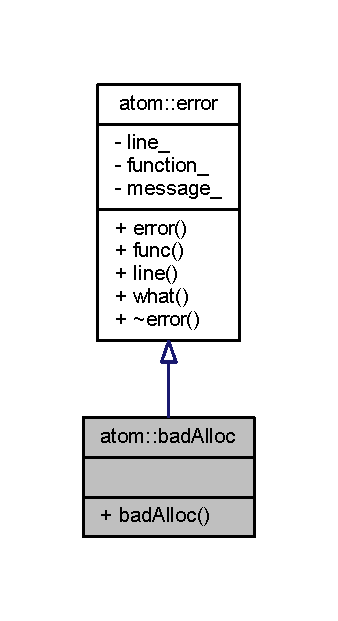
\includegraphics[width=162pt]{classatom_1_1bad_alloc__inherit__graph}
\end{center}
\end{figure}


Collaboration diagram for atom\+:\+:bad\+Alloc\+:
\nopagebreak
\begin{figure}[H]
\begin{center}
\leavevmode
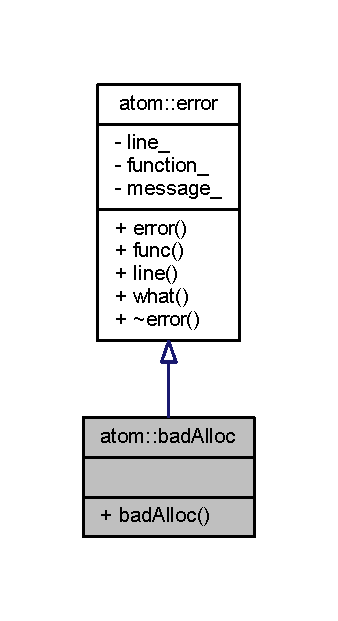
\includegraphics[width=162pt]{classatom_1_1bad_alloc__coll__graph}
\end{center}
\end{figure}
\subsection*{Public Member Functions}
\begin{DoxyCompactItemize}
\item 
\mbox{\Hypertarget{classatom_1_1bad_alloc_afcf798fbb60d759728033cd30c01b0e8}\label{classatom_1_1bad_alloc_afcf798fbb60d759728033cd30c01b0e8}} 
{\bfseries bad\+Alloc} (\hyperlink{classatom_1_1error_ac330e9fb7cedcf4a173c5eb156d7bdaf}{const\+\_\+string\+\_\+type} \&\hyperlink{classatom_1_1error_a0a70a92b1638bfe4be7972651ae0c5c8}{func}=\char`\"{}\char`\"{}, const int \hyperlink{classatom_1_1error_aa9443d1a458d0dc6086372444a58e8c6}{line}=0, \hyperlink{classatom_1_1error_ac330e9fb7cedcf4a173c5eb156d7bdaf}{const\+\_\+string\+\_\+type} \&msg=\char`\"{}\char`\"{})
\end{DoxyCompactItemize}
\subsection*{Additional Inherited Members}


\subsection{Detailed Description}
Exception about problems with allocate of the memory. 

Derived from class error 

The documentation for this class was generated from the following file\+:\begin{DoxyCompactItemize}
\item 
D\+:/\+Git\+Hub/\+Techno\+Atom/src/\hyperlink{exceptions_8h}{exceptions.\+h}\end{DoxyCompactItemize}

\hypertarget{classatom_1_1error}{}\section{atom\+:\+:error Class Reference}
\label{classatom_1_1error}\index{atom\+::error@{atom\+::error}}


Abstract class which is template for all exceptions.  




{\ttfamily \#include $<$exceptions.\+h$>$}



Inheritance diagram for atom\+:\+:error\+:
\nopagebreak
\begin{figure}[H]
\begin{center}
\leavevmode
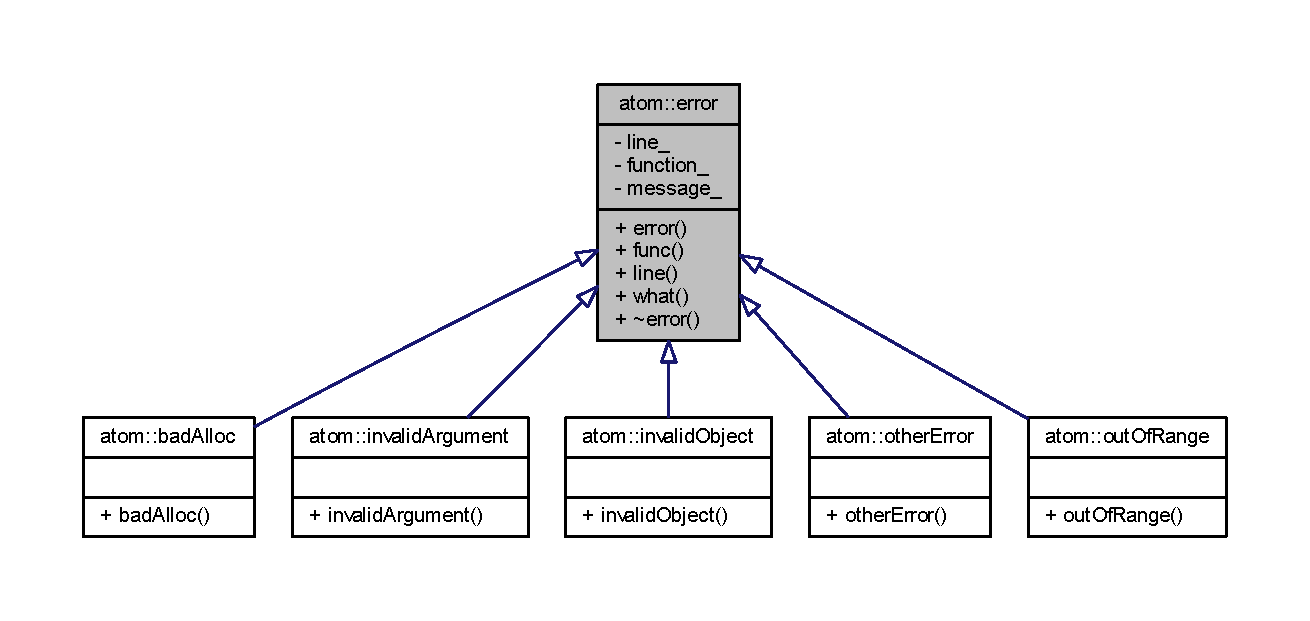
\includegraphics[width=350pt]{classatom_1_1error__inherit__graph}
\end{center}
\end{figure}


Collaboration diagram for atom\+:\+:error\+:
\nopagebreak
\begin{figure}[H]
\begin{center}
\leavevmode
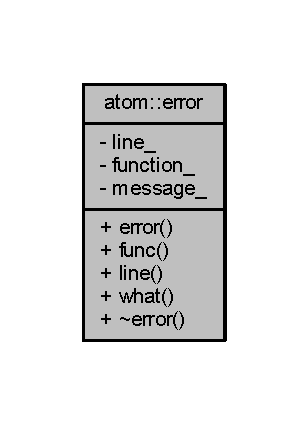
\includegraphics[width=148pt]{classatom_1_1error__coll__graph}
\end{center}
\end{figure}
\subsection*{Public Types}
\begin{DoxyCompactItemize}
\item 
\mbox{\Hypertarget{classatom_1_1error_ac330e9fb7cedcf4a173c5eb156d7bdaf}\label{classatom_1_1error_ac330e9fb7cedcf4a173c5eb156d7bdaf}} 
using \hyperlink{classatom_1_1error_ac330e9fb7cedcf4a173c5eb156d7bdaf}{const\+\_\+string\+\_\+type} = const std\+::string
\begin{DoxyCompactList}\small\item\em Const string type. \end{DoxyCompactList}\end{DoxyCompactItemize}
\subsection*{Public Member Functions}
\begin{DoxyCompactItemize}
\item 
\hyperlink{classatom_1_1error_aef6fb75c74af10599648f701cf8b0844}{error} (\hyperlink{classatom_1_1error_ac330e9fb7cedcf4a173c5eb156d7bdaf}{const\+\_\+string\+\_\+type} \&\hyperlink{classatom_1_1error_a0a70a92b1638bfe4be7972651ae0c5c8}{func}=\char`\"{}\char`\"{}, const int \hyperlink{classatom_1_1error_aa9443d1a458d0dc6086372444a58e8c6}{line}=0, \hyperlink{classatom_1_1error_ac330e9fb7cedcf4a173c5eb156d7bdaf}{const\+\_\+string\+\_\+type} \&msg=\char`\"{}\char`\"{})
\item 
\hyperlink{classatom_1_1error_ac330e9fb7cedcf4a173c5eb156d7bdaf}{const\+\_\+string\+\_\+type} \hyperlink{classatom_1_1error_a0a70a92b1638bfe4be7972651ae0c5c8}{func} () const
\item 
int \hyperlink{classatom_1_1error_aa9443d1a458d0dc6086372444a58e8c6}{line} () const
\item 
\hyperlink{classatom_1_1error_ac330e9fb7cedcf4a173c5eb156d7bdaf}{const\+\_\+string\+\_\+type} \hyperlink{classatom_1_1error_a126f6c573e37febac3148244389f7736}{what} () const
\item 
virtual \hyperlink{classatom_1_1error_a89bbb11a0ab57de79697ad10e64a77fb}{$\sim$error} ()=0
\end{DoxyCompactItemize}
\subsection*{Private Attributes}
\begin{DoxyCompactItemize}
\item 
\mbox{\Hypertarget{classatom_1_1error_a8f9a09becabf82e9c407835b310fada8}\label{classatom_1_1error_a8f9a09becabf82e9c407835b310fada8}} 
const int \hyperlink{classatom_1_1error_a8f9a09becabf82e9c407835b310fada8}{line\+\_\+}
\begin{DoxyCompactList}\small\item\em Number of the line. \end{DoxyCompactList}\item 
\mbox{\Hypertarget{classatom_1_1error_ad0c225c85dd50d88097448212e0f513a}\label{classatom_1_1error_ad0c225c85dd50d88097448212e0f513a}} 
\hyperlink{classatom_1_1error_ac330e9fb7cedcf4a173c5eb156d7bdaf}{const\+\_\+string\+\_\+type} \hyperlink{classatom_1_1error_ad0c225c85dd50d88097448212e0f513a}{function\+\_\+}
\begin{DoxyCompactList}\small\item\em Name of the function which generate exception. \end{DoxyCompactList}\item 
\mbox{\Hypertarget{classatom_1_1error_a0c32da54f099b6adb57033f21660e04d}\label{classatom_1_1error_a0c32da54f099b6adb57033f21660e04d}} 
\hyperlink{classatom_1_1error_ac330e9fb7cedcf4a173c5eb156d7bdaf}{const\+\_\+string\+\_\+type} \hyperlink{classatom_1_1error_a0c32da54f099b6adb57033f21660e04d}{message\+\_\+}
\begin{DoxyCompactList}\small\item\em Additional messange about error. \end{DoxyCompactList}\end{DoxyCompactItemize}


\subsection{Detailed Description}
Abstract class which is template for all exceptions. 

Have three members\+: function\+\_\+, line\+\_\+, message\+\_\+

which discribe place where was generate exception and give message about it 

\subsection{Constructor \& Destructor Documentation}
\mbox{\Hypertarget{classatom_1_1error_aef6fb75c74af10599648f701cf8b0844}\label{classatom_1_1error_aef6fb75c74af10599648f701cf8b0844}} 
\index{atom\+::error@{atom\+::error}!error@{error}}
\index{error@{error}!atom\+::error@{atom\+::error}}
\subsubsection{\texorpdfstring{error()}{error()}}
{\footnotesize\ttfamily atom\+::error\+::error (\begin{DoxyParamCaption}\item[{\hyperlink{classatom_1_1error_ac330e9fb7cedcf4a173c5eb156d7bdaf}{const\+\_\+string\+\_\+type} \&}]{func = {\ttfamily \char`\"{}\char`\"{}},  }\item[{const int}]{line = {\ttfamily 0},  }\item[{\hyperlink{classatom_1_1error_ac330e9fb7cedcf4a173c5eb156d7bdaf}{const\+\_\+string\+\_\+type} \&}]{msg = {\ttfamily \char`\"{}\char`\"{}} }\end{DoxyParamCaption})\hspace{0.3cm}{\ttfamily [inline]}}

Constructor 
\begin{DoxyParams}{Parameters}
{\em func} & Name of the function which generate exception \\
\hline
{\em line} & Number of the line \\
\hline
{\em msg} & Additional messange about error \\
\hline
\end{DoxyParams}
\mbox{\Hypertarget{classatom_1_1error_a89bbb11a0ab57de79697ad10e64a77fb}\label{classatom_1_1error_a89bbb11a0ab57de79697ad10e64a77fb}} 
\index{atom\+::error@{atom\+::error}!````~error@{$\sim$error}}
\index{````~error@{$\sim$error}!atom\+::error@{atom\+::error}}
\subsubsection{\texorpdfstring{$\sim$error()}{~error()}}
{\footnotesize\ttfamily atom\+::error\+::$\sim$error (\begin{DoxyParamCaption}{ }\end{DoxyParamCaption})\hspace{0.3cm}{\ttfamily [pure virtual]}}

Pure virtual destructor

With the aim of abstraction of the class 

\subsection{Member Function Documentation}
\mbox{\Hypertarget{classatom_1_1error_a0a70a92b1638bfe4be7972651ae0c5c8}\label{classatom_1_1error_a0a70a92b1638bfe4be7972651ae0c5c8}} 
\index{atom\+::error@{atom\+::error}!func@{func}}
\index{func@{func}!atom\+::error@{atom\+::error}}
\subsubsection{\texorpdfstring{func()}{func()}}
{\footnotesize\ttfamily \hyperlink{classatom_1_1error_ac330e9fb7cedcf4a173c5eb156d7bdaf}{const\+\_\+string\+\_\+type} atom\+::error\+::func (\begin{DoxyParamCaption}{ }\end{DoxyParamCaption}) const\hspace{0.3cm}{\ttfamily [inline]}}

Return name caused function  const std\+::string -\/ name function \mbox{\Hypertarget{classatom_1_1error_aa9443d1a458d0dc6086372444a58e8c6}\label{classatom_1_1error_aa9443d1a458d0dc6086372444a58e8c6}} 
\index{atom\+::error@{atom\+::error}!line@{line}}
\index{line@{line}!atom\+::error@{atom\+::error}}
\subsubsection{\texorpdfstring{line()}{line()}}
{\footnotesize\ttfamily int atom\+::error\+::line (\begin{DoxyParamCaption}{ }\end{DoxyParamCaption}) const\hspace{0.3cm}{\ttfamily [inline]}}

Return number line where was exception \begin{DoxyReturn}{Returns}
number of the line 
\end{DoxyReturn}
\mbox{\Hypertarget{classatom_1_1error_a126f6c573e37febac3148244389f7736}\label{classatom_1_1error_a126f6c573e37febac3148244389f7736}} 
\index{atom\+::error@{atom\+::error}!what@{what}}
\index{what@{what}!atom\+::error@{atom\+::error}}
\subsubsection{\texorpdfstring{what()}{what()}}
{\footnotesize\ttfamily \hyperlink{classatom_1_1error_ac330e9fb7cedcf4a173c5eb156d7bdaf}{const\+\_\+string\+\_\+type} atom\+::error\+::what (\begin{DoxyParamCaption}{ }\end{DoxyParamCaption}) const\hspace{0.3cm}{\ttfamily [inline]}}

Message about error \begin{DoxyReturn}{Returns}
const std\+::string -\/ message 
\end{DoxyReturn}


The documentation for this class was generated from the following file\+:\begin{DoxyCompactItemize}
\item 
D\+:/\+Git\+Hub/\+Techno\+Atom/task 2/src/\hyperlink{exceptions_8h}{exceptions.\+h}\end{DoxyCompactItemize}

\hypertarget{classatom_1_1invalid_argument}{}\section{atom\+:\+:invalid\+Argument Class Reference}
\label{classatom_1_1invalid_argument}\index{atom\+::invalid\+Argument@{atom\+::invalid\+Argument}}


Exception about problems with arguments in functions.  




{\ttfamily \#include $<$exceptions.\+h$>$}



Inheritance diagram for atom\+:\+:invalid\+Argument\+:
\nopagebreak
\begin{figure}[H]
\begin{center}
\leavevmode
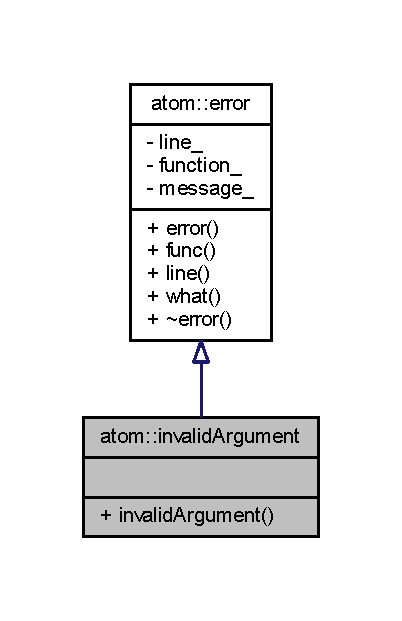
\includegraphics[width=193pt]{classatom_1_1invalid_argument__inherit__graph}
\end{center}
\end{figure}


Collaboration diagram for atom\+:\+:invalid\+Argument\+:
\nopagebreak
\begin{figure}[H]
\begin{center}
\leavevmode
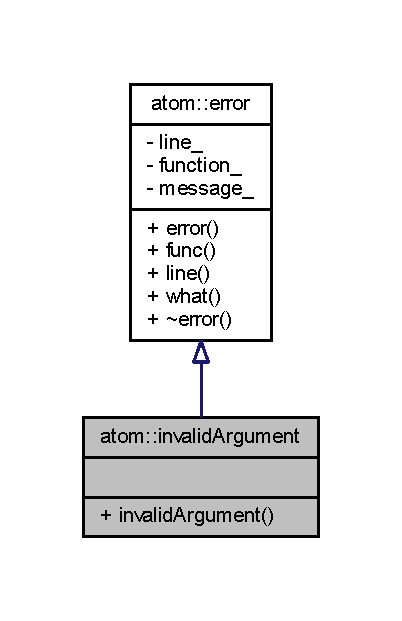
\includegraphics[width=193pt]{classatom_1_1invalid_argument__coll__graph}
\end{center}
\end{figure}
\subsection*{Public Member Functions}
\begin{DoxyCompactItemize}
\item 
\mbox{\Hypertarget{classatom_1_1invalid_argument_a21255e405e4aa56098092b4ac75d53e4}\label{classatom_1_1invalid_argument_a21255e405e4aa56098092b4ac75d53e4}} 
{\bfseries invalid\+Argument} (\hyperlink{classatom_1_1error_ac330e9fb7cedcf4a173c5eb156d7bdaf}{const\+\_\+string\+\_\+type} \&\hyperlink{classatom_1_1error_a0a70a92b1638bfe4be7972651ae0c5c8}{func}=\char`\"{}\char`\"{}, const int \hyperlink{classatom_1_1error_aa9443d1a458d0dc6086372444a58e8c6}{line}=0, \hyperlink{classatom_1_1error_ac330e9fb7cedcf4a173c5eb156d7bdaf}{const\+\_\+string\+\_\+type} \&msg=\char`\"{}\char`\"{})
\end{DoxyCompactItemize}
\subsection*{Additional Inherited Members}


\subsection{Detailed Description}
Exception about problems with arguments in functions. 

Derived from class error 

The documentation for this class was generated from the following file\+:\begin{DoxyCompactItemize}
\item 
D\+:/\+Git\+Hub/\+Techno\+Atom/task 2/src/\hyperlink{exceptions_8h}{exceptions.\+h}\end{DoxyCompactItemize}

\hypertarget{classatom_1_1invalid_object}{}\section{atom\+:\+:invalid\+Object Class Reference}
\label{classatom_1_1invalid_object}\index{atom\+::invalid\+Object@{atom\+::invalid\+Object}}


Exception about problems with object different classes.  




{\ttfamily \#include $<$exceptions.\+h$>$}



Inheritance diagram for atom\+:\+:invalid\+Object\+:
\nopagebreak
\begin{figure}[H]
\begin{center}
\leavevmode
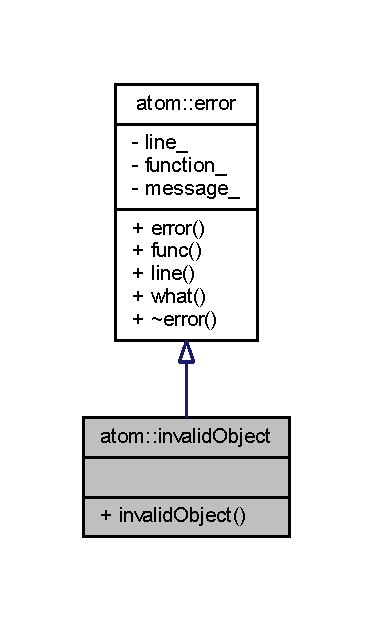
\includegraphics[width=179pt]{classatom_1_1invalid_object__inherit__graph}
\end{center}
\end{figure}


Collaboration diagram for atom\+:\+:invalid\+Object\+:
\nopagebreak
\begin{figure}[H]
\begin{center}
\leavevmode
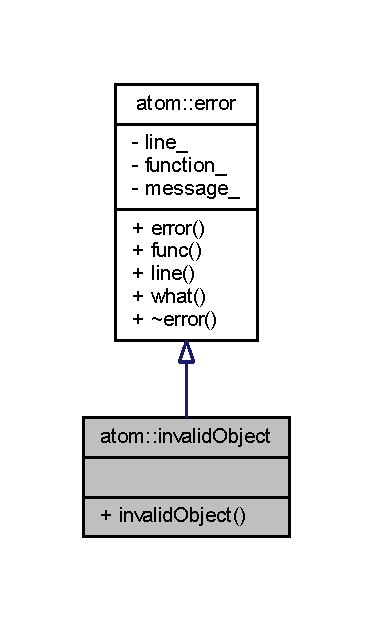
\includegraphics[width=179pt]{classatom_1_1invalid_object__coll__graph}
\end{center}
\end{figure}
\subsection*{Public Member Functions}
\begin{DoxyCompactItemize}
\item 
\mbox{\Hypertarget{classatom_1_1invalid_object_a70f97b01ac566e63753ee29e6e862228}\label{classatom_1_1invalid_object_a70f97b01ac566e63753ee29e6e862228}} 
{\bfseries invalid\+Object} (\hyperlink{classatom_1_1error_ac330e9fb7cedcf4a173c5eb156d7bdaf}{const\+\_\+string\+\_\+type} \&\hyperlink{classatom_1_1error_a0a70a92b1638bfe4be7972651ae0c5c8}{func}=\char`\"{}\char`\"{}, const int \hyperlink{classatom_1_1error_aa9443d1a458d0dc6086372444a58e8c6}{line}=0, \hyperlink{classatom_1_1error_ac330e9fb7cedcf4a173c5eb156d7bdaf}{const\+\_\+string\+\_\+type} \&msg=\char`\"{}\char`\"{})
\end{DoxyCompactItemize}
\subsection*{Additional Inherited Members}


\subsection{Detailed Description}
Exception about problems with object different classes. 

Derived from class error 

The documentation for this class was generated from the following file\+:\begin{DoxyCompactItemize}
\item 
D\+:/\+Git\+Hub/\+Techno\+Atom/task 2/src/\hyperlink{exceptions_8h}{exceptions.\+h}\end{DoxyCompactItemize}

\hypertarget{classatom_1_1other_error}{}\section{atom\+:\+:other\+Error Class Reference}
\label{classatom_1_1other_error}\index{atom\+::other\+Error@{atom\+::other\+Error}}


Undefine here exceptions.  




{\ttfamily \#include $<$exceptions.\+h$>$}



Inheritance diagram for atom\+:\+:other\+Error\+:
\nopagebreak
\begin{figure}[H]
\begin{center}
\leavevmode
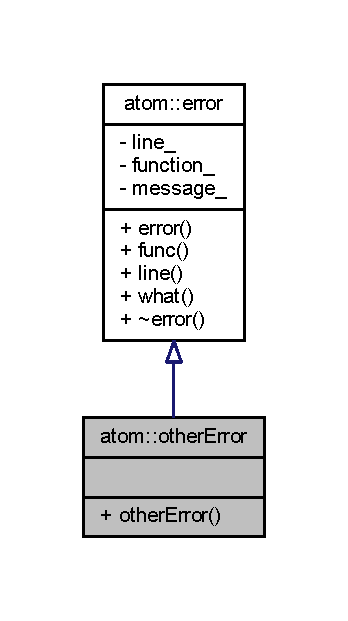
\includegraphics[width=167pt]{classatom_1_1other_error__inherit__graph}
\end{center}
\end{figure}


Collaboration diagram for atom\+:\+:other\+Error\+:
\nopagebreak
\begin{figure}[H]
\begin{center}
\leavevmode
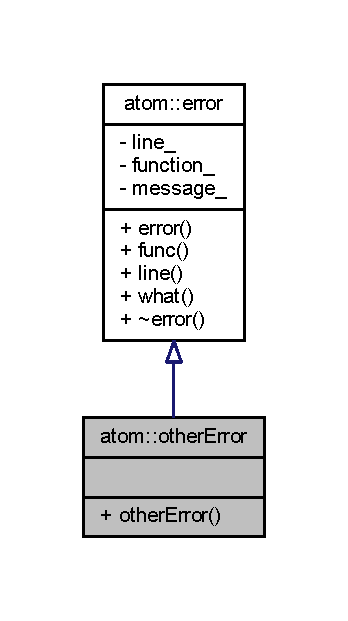
\includegraphics[width=167pt]{classatom_1_1other_error__coll__graph}
\end{center}
\end{figure}
\subsection*{Public Member Functions}
\begin{DoxyCompactItemize}
\item 
\mbox{\Hypertarget{classatom_1_1other_error_a55d13dbae6599e17d7aa07afab4a40d3}\label{classatom_1_1other_error_a55d13dbae6599e17d7aa07afab4a40d3}} 
{\bfseries other\+Error} (\hyperlink{classatom_1_1error_ac330e9fb7cedcf4a173c5eb156d7bdaf}{const\+\_\+string\+\_\+type} \&\hyperlink{classatom_1_1error_a0a70a92b1638bfe4be7972651ae0c5c8}{func}=\char`\"{}\char`\"{}, const int \hyperlink{classatom_1_1error_aa9443d1a458d0dc6086372444a58e8c6}{line}=0, \hyperlink{classatom_1_1error_ac330e9fb7cedcf4a173c5eb156d7bdaf}{const\+\_\+string\+\_\+type} \&msg=\char`\"{}\char`\"{})
\end{DoxyCompactItemize}
\subsection*{Additional Inherited Members}


\subsection{Detailed Description}
Undefine here exceptions. 

Derived from class error 

The documentation for this class was generated from the following file\+:\begin{DoxyCompactItemize}
\item 
D\+:/\+Git\+Hub/\+Techno\+Atom/src/\hyperlink{exceptions_8h}{exceptions.\+h}\end{DoxyCompactItemize}

\hypertarget{classatom_1_1out_of_range}{}\section{atom\+:\+:out\+Of\+Range Class Reference}
\label{classatom_1_1out_of_range}\index{atom\+::out\+Of\+Range@{atom\+::out\+Of\+Range}}


Exception about problems connected with borders.  




{\ttfamily \#include $<$exceptions.\+h$>$}



Inheritance diagram for atom\+:\+:out\+Of\+Range\+:
\nopagebreak
\begin{figure}[H]
\begin{center}
\leavevmode
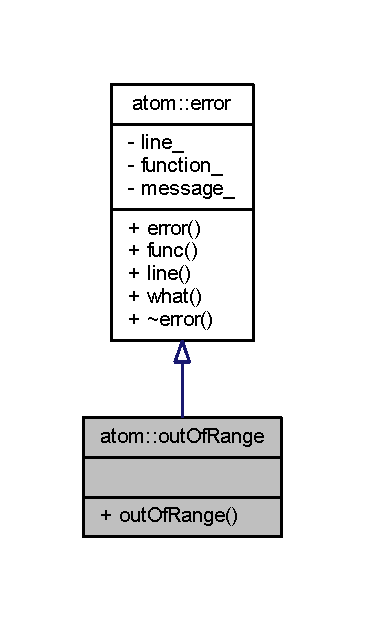
\includegraphics[width=175pt]{classatom_1_1out_of_range__inherit__graph}
\end{center}
\end{figure}


Collaboration diagram for atom\+:\+:out\+Of\+Range\+:
\nopagebreak
\begin{figure}[H]
\begin{center}
\leavevmode
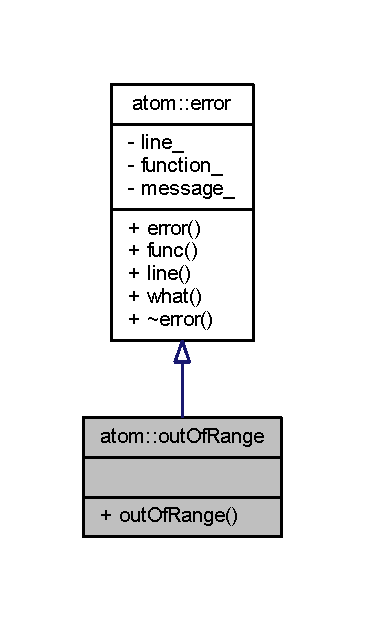
\includegraphics[width=175pt]{classatom_1_1out_of_range__coll__graph}
\end{center}
\end{figure}
\subsection*{Public Member Functions}
\begin{DoxyCompactItemize}
\item 
\mbox{\Hypertarget{classatom_1_1out_of_range_a388ec1d8924de5cfdc8b3bf06554fb3d}\label{classatom_1_1out_of_range_a388ec1d8924de5cfdc8b3bf06554fb3d}} 
{\bfseries out\+Of\+Range} (\hyperlink{classatom_1_1error_ac330e9fb7cedcf4a173c5eb156d7bdaf}{const\+\_\+string\+\_\+type} \&\hyperlink{classatom_1_1error_a0a70a92b1638bfe4be7972651ae0c5c8}{func}=\char`\"{}\char`\"{}, const int \hyperlink{classatom_1_1error_aa9443d1a458d0dc6086372444a58e8c6}{line}=0, \hyperlink{classatom_1_1error_ac330e9fb7cedcf4a173c5eb156d7bdaf}{const\+\_\+string\+\_\+type} \&msg=\char`\"{}\char`\"{})
\end{DoxyCompactItemize}
\subsection*{Additional Inherited Members}


\subsection{Detailed Description}
Exception about problems connected with borders. 

Derived from class error 

The documentation for this class was generated from the following file\+:\begin{DoxyCompactItemize}
\item 
D\+:/\+Git\+Hub/\+Techno\+Atom/src/\hyperlink{exceptions_8h}{exceptions.\+h}\end{DoxyCompactItemize}

\hypertarget{struct_p_o_i_s_o_n}{}\section{P\+O\+I\+S\+ON$<$ Tp $>$ Struct Template Reference}
\label{struct_p_o_i_s_o_n}\index{P\+O\+I\+S\+O\+N$<$ Tp $>$@{P\+O\+I\+S\+O\+N$<$ Tp $>$}}


Poison constant for any elements.  




{\ttfamily \#include $<$debug\+\_\+tools.\+h$>$}



Collaboration diagram for P\+O\+I\+S\+ON$<$ Tp $>$\+:
\nopagebreak
\begin{figure}[H]
\begin{center}
\leavevmode
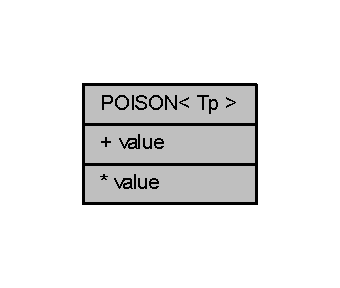
\includegraphics[width=163pt]{struct_p_o_i_s_o_n__coll__graph}
\end{center}
\end{figure}
\subsection*{Static Public Attributes}
\textbf{ }\par
\begin{DoxyCompactItemize}
\item 
\mbox{\Hypertarget{struct_p_o_i_s_o_n_a75c30e11745e5ccf77df2b30ad3bb1f3}\label{struct_p_o_i_s_o_n_a75c30e11745e5ccf77df2b30ad3bb1f3}} 
static const Tp \hyperlink{struct_p_o_i_s_o_n_a75c30e11745e5ccf77df2b30ad3bb1f3}{value} = Tp()
\begin{DoxyCompactList}\small\item\em List of all poisons. \end{DoxyCompactList}\end{DoxyCompactItemize}



\subsection{Detailed Description}
\subsubsection*{template$<$typename Tp$>$\newline
struct P\+O\+I\+S\+O\+N$<$ Tp $>$}

Poison constant for any elements. 

Poison constant for unsigned long long elements.

Poison constant for long long elements.

Poison constant for unsigned char elements.

Poison constant for char elements.

Poison constant for double elements.

Poison constant for float elements.

Poison constant for unsigned int elements.

Poison constant for int elements.

Poison constant for unsigned short elements.

Poison constant for short elements.


\begin{DoxyTemplParams}{Template Parameters}
{\em Tp} & The type of data used \\
\hline
\end{DoxyTemplParams}


The documentation for this struct was generated from the following file\+:\begin{DoxyCompactItemize}
\item 
D\+:/\+Git\+Hub/\+Techno\+Atom/src/\hyperlink{debug__tools_8h}{debug\+\_\+tools.\+h}\end{DoxyCompactItemize}

\hypertarget{struct_p_o_i_s_o_n_3_01char_01_4}{}\section{P\+O\+I\+S\+ON$<$ char $>$ Struct Template Reference}
\label{struct_p_o_i_s_o_n_3_01char_01_4}\index{P\+O\+I\+S\+O\+N$<$ char $>$@{P\+O\+I\+S\+O\+N$<$ char $>$}}


Collaboration diagram for P\+O\+I\+S\+ON$<$ char $>$\+:
\nopagebreak
\begin{figure}[H]
\begin{center}
\leavevmode
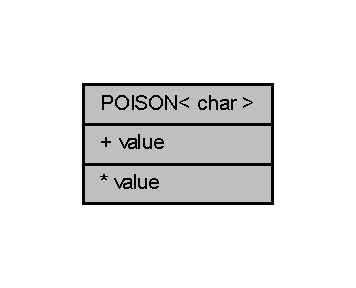
\includegraphics[width=171pt]{struct_p_o_i_s_o_n_3_01char_01_4__coll__graph}
\end{center}
\end{figure}
\subsection*{Static Public Attributes}
\textbf{ }\par
\begin{DoxyCompactItemize}
\item 
\mbox{\Hypertarget{struct_p_o_i_s_o_n_3_01char_01_4_aa67110240ea4d4906071479b36c3f7e3}\label{struct_p_o_i_s_o_n_3_01char_01_4_aa67110240ea4d4906071479b36c3f7e3}} 
static const char {\bfseries value} = static\+\_\+cast$<$char$>$(-\/12)
\end{DoxyCompactItemize}



The documentation for this struct was generated from the following file\+:\begin{DoxyCompactItemize}
\item 
D\+:/\+Git\+Hub/\+Techno\+Atom/task 2/src/\hyperlink{debug__tools_8h}{debug\+\_\+tools.\+h}\end{DoxyCompactItemize}

\hypertarget{struct_p_o_i_s_o_n_3_01double_01_4}{}\section{P\+O\+I\+S\+ON$<$ double $>$ Struct Template Reference}
\label{struct_p_o_i_s_o_n_3_01double_01_4}\index{P\+O\+I\+S\+O\+N$<$ double $>$@{P\+O\+I\+S\+O\+N$<$ double $>$}}


Collaboration diagram for P\+O\+I\+S\+ON$<$ double $>$\+:
\nopagebreak
\begin{figure}[H]
\begin{center}
\leavevmode
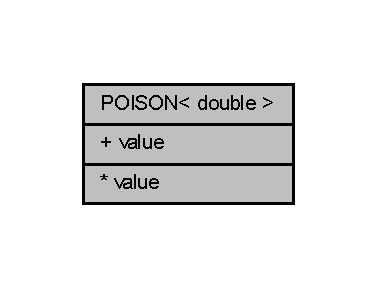
\includegraphics[width=181pt]{struct_p_o_i_s_o_n_3_01double_01_4__coll__graph}
\end{center}
\end{figure}
\subsection*{Static Public Attributes}
\textbf{ }\par
\begin{DoxyCompactItemize}
\item 
\mbox{\Hypertarget{struct_p_o_i_s_o_n_3_01double_01_4_aa06e0aac29e46b6fc449dfddad0bba91}\label{struct_p_o_i_s_o_n_3_01double_01_4_aa06e0aac29e46b6fc449dfddad0bba91}} 
static const double {\bfseries value} = 2588511426\+E-\/7
\end{DoxyCompactItemize}



The documentation for this struct was generated from the following file\+:\begin{DoxyCompactItemize}
\item 
D\+:/\+Git\+Hub/\+Techno\+Atom/src/\hyperlink{debug__tools_8h}{debug\+\_\+tools.\+h}\end{DoxyCompactItemize}

\hypertarget{struct_p_o_i_s_o_n_3_01float_01_4}{}\section{P\+O\+I\+S\+ON$<$ float $>$ Struct Template Reference}
\label{struct_p_o_i_s_o_n_3_01float_01_4}\index{P\+O\+I\+S\+O\+N$<$ float $>$@{P\+O\+I\+S\+O\+N$<$ float $>$}}


Collaboration diagram for P\+O\+I\+S\+ON$<$ float $>$\+:
\nopagebreak
\begin{figure}[H]
\begin{center}
\leavevmode
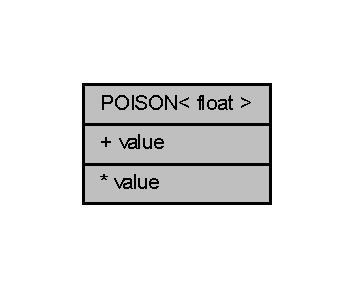
\includegraphics[width=170pt]{struct_p_o_i_s_o_n_3_01float_01_4__coll__graph}
\end{center}
\end{figure}
\subsection*{Static Public Attributes}
\textbf{ }\par
\begin{DoxyCompactItemize}
\item 
\mbox{\Hypertarget{struct_p_o_i_s_o_n_3_01float_01_4_af865aaa1259e02b92b1d32bb981ce065}\label{struct_p_o_i_s_o_n_3_01float_01_4_af865aaa1259e02b92b1d32bb981ce065}} 
static const float {\bfseries value} = -\/722004.\+5482f
\end{DoxyCompactItemize}



The documentation for this struct was generated from the following file\+:\begin{DoxyCompactItemize}
\item 
D\+:/\+Git\+Hub/\+Techno\+Atom/task 2/src/\hyperlink{debug__tools_8h}{debug\+\_\+tools.\+h}\end{DoxyCompactItemize}

\hypertarget{struct_p_o_i_s_o_n_3_01int_01_4}{}\section{P\+O\+I\+S\+ON$<$ int $>$ Struct Template Reference}
\label{struct_p_o_i_s_o_n_3_01int_01_4}\index{P\+O\+I\+S\+O\+N$<$ int $>$@{P\+O\+I\+S\+O\+N$<$ int $>$}}


Collaboration diagram for P\+O\+I\+S\+ON$<$ int $>$\+:
\nopagebreak
\begin{figure}[H]
\begin{center}
\leavevmode
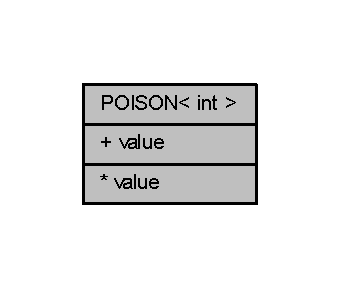
\includegraphics[width=163pt]{struct_p_o_i_s_o_n_3_01int_01_4__coll__graph}
\end{center}
\end{figure}
\subsection*{Static Public Attributes}
\textbf{ }\par
\begin{DoxyCompactItemize}
\item 
\mbox{\Hypertarget{struct_p_o_i_s_o_n_3_01int_01_4_a4a7b41de4a6a4e91119dc2bfab15ba07}\label{struct_p_o_i_s_o_n_3_01int_01_4_a4a7b41de4a6a4e91119dc2bfab15ba07}} 
static const int {\bfseries value} = -\/8631004
\end{DoxyCompactItemize}



The documentation for this struct was generated from the following file\+:\begin{DoxyCompactItemize}
\item 
D\+:/\+Git\+Hub/\+Techno\+Atom/task 2/src/\hyperlink{debug__tools_8h}{debug\+\_\+tools.\+h}\end{DoxyCompactItemize}

\hypertarget{struct_p_o_i_s_o_n_3_01long_01long_01_4}{}\section{P\+O\+I\+S\+ON$<$ long long $>$ Struct Template Reference}
\label{struct_p_o_i_s_o_n_3_01long_01long_01_4}\index{P\+O\+I\+S\+O\+N$<$ long long $>$@{P\+O\+I\+S\+O\+N$<$ long long $>$}}


Collaboration diagram for P\+O\+I\+S\+ON$<$ long long $>$\+:
\nopagebreak
\begin{figure}[H]
\begin{center}
\leavevmode
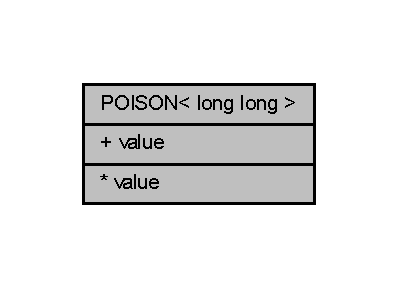
\includegraphics[width=191pt]{struct_p_o_i_s_o_n_3_01long_01long_01_4__coll__graph}
\end{center}
\end{figure}
\subsection*{Static Public Attributes}
\textbf{ }\par
\begin{DoxyCompactItemize}
\item 
\mbox{\Hypertarget{struct_p_o_i_s_o_n_3_01long_01long_01_4_a92c6c904c4763d3f39cd904cada4ec44}\label{struct_p_o_i_s_o_n_3_01long_01long_01_4_a92c6c904c4763d3f39cd904cada4ec44}} 
static const long long {\bfseries value} = -\/147520069954\+LL
\end{DoxyCompactItemize}



The documentation for this struct was generated from the following file\+:\begin{DoxyCompactItemize}
\item 
D\+:/\+Git\+Hub/\+Techno\+Atom/src/\hyperlink{debug__tools_8h}{debug\+\_\+tools.\+h}\end{DoxyCompactItemize}

\hypertarget{struct_p_o_i_s_o_n_3_01short_01_4}{}\section{P\+O\+I\+S\+ON$<$ short $>$ Struct Template Reference}
\label{struct_p_o_i_s_o_n_3_01short_01_4}\index{P\+O\+I\+S\+O\+N$<$ short $>$@{P\+O\+I\+S\+O\+N$<$ short $>$}}


Collaboration diagram for P\+O\+I\+S\+ON$<$ short $>$\+:
\nopagebreak
\begin{figure}[H]
\begin{center}
\leavevmode
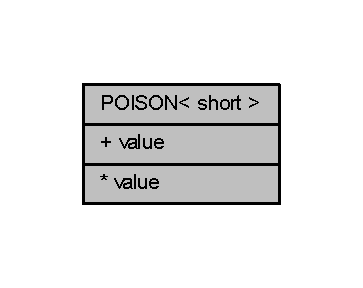
\includegraphics[width=174pt]{struct_p_o_i_s_o_n_3_01short_01_4__coll__graph}
\end{center}
\end{figure}
\subsection*{Static Public Attributes}
\textbf{ }\par
\begin{DoxyCompactItemize}
\item 
\mbox{\Hypertarget{struct_p_o_i_s_o_n_3_01short_01_4_a01dfef4676ecb3ae01b25c8e239d7d7f}\label{struct_p_o_i_s_o_n_3_01short_01_4_a01dfef4676ecb3ae01b25c8e239d7d7f}} 
static const short {\bfseries value} = -\/121
\end{DoxyCompactItemize}



The documentation for this struct was generated from the following file\+:\begin{DoxyCompactItemize}
\item 
D\+:/\+Git\+Hub/\+Techno\+Atom/task 2/src/\hyperlink{debug__tools_8h}{debug\+\_\+tools.\+h}\end{DoxyCompactItemize}

\hypertarget{struct_p_o_i_s_o_n_3_01unsigned_01char_01_4}{}\section{P\+O\+I\+S\+ON$<$ unsigned char $>$ Struct Template Reference}
\label{struct_p_o_i_s_o_n_3_01unsigned_01char_01_4}\index{P\+O\+I\+S\+O\+N$<$ unsigned char $>$@{P\+O\+I\+S\+O\+N$<$ unsigned char $>$}}


Collaboration diagram for P\+O\+I\+S\+ON$<$ unsigned char $>$\+:
\nopagebreak
\begin{figure}[H]
\begin{center}
\leavevmode
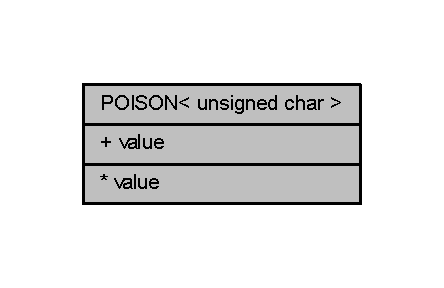
\includegraphics[width=213pt]{struct_p_o_i_s_o_n_3_01unsigned_01char_01_4__coll__graph}
\end{center}
\end{figure}
\subsection*{Static Public Attributes}
\textbf{ }\par
\begin{DoxyCompactItemize}
\item 
\mbox{\Hypertarget{struct_p_o_i_s_o_n_3_01unsigned_01char_01_4_a7d966240ad6bf556979b7f6c8fecfd37}\label{struct_p_o_i_s_o_n_3_01unsigned_01char_01_4_a7d966240ad6bf556979b7f6c8fecfd37}} 
static const unsigned char {\bfseries value} = static\+\_\+cast$<$unsigned char$>$(12)
\end{DoxyCompactItemize}



The documentation for this struct was generated from the following file\+:\begin{DoxyCompactItemize}
\item 
D\+:/\+Git\+Hub/\+Techno\+Atom/task 2/src/\hyperlink{debug__tools_8h}{debug\+\_\+tools.\+h}\end{DoxyCompactItemize}

\hypertarget{struct_p_o_i_s_o_n_3_01unsigned_01int_01_4}{}\section{P\+O\+I\+S\+ON$<$ unsigned int $>$ Struct Template Reference}
\label{struct_p_o_i_s_o_n_3_01unsigned_01int_01_4}\index{P\+O\+I\+S\+O\+N$<$ unsigned int $>$@{P\+O\+I\+S\+O\+N$<$ unsigned int $>$}}


Collaboration diagram for P\+O\+I\+S\+ON$<$ unsigned int $>$\+:
\nopagebreak
\begin{figure}[H]
\begin{center}
\leavevmode
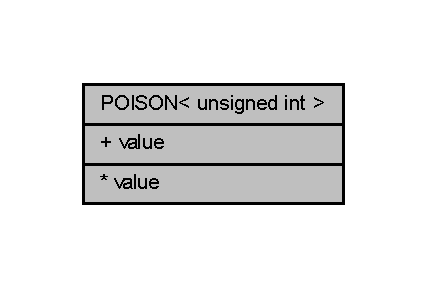
\includegraphics[width=205pt]{struct_p_o_i_s_o_n_3_01unsigned_01int_01_4__coll__graph}
\end{center}
\end{figure}
\subsection*{Static Public Attributes}
\textbf{ }\par
\begin{DoxyCompactItemize}
\item 
\mbox{\Hypertarget{struct_p_o_i_s_o_n_3_01unsigned_01int_01_4_a5f0e085925546c8f4cd331922253dcbe}\label{struct_p_o_i_s_o_n_3_01unsigned_01int_01_4_a5f0e085925546c8f4cd331922253dcbe}} 
static const unsigned int {\bfseries value} = 8631004u
\end{DoxyCompactItemize}



The documentation for this struct was generated from the following file\+:\begin{DoxyCompactItemize}
\item 
D\+:/\+Git\+Hub/\+Techno\+Atom/task 2/src/\hyperlink{debug__tools_8h}{debug\+\_\+tools.\+h}\end{DoxyCompactItemize}

\hypertarget{struct_p_o_i_s_o_n_3_01unsigned_01long_01long_01_4}{}\section{P\+O\+I\+S\+ON$<$ unsigned long long $>$ Struct Template Reference}
\label{struct_p_o_i_s_o_n_3_01unsigned_01long_01long_01_4}\index{P\+O\+I\+S\+O\+N$<$ unsigned long long $>$@{P\+O\+I\+S\+O\+N$<$ unsigned long long $>$}}


Collaboration diagram for P\+O\+I\+S\+ON$<$ unsigned long long $>$\+:
\nopagebreak
\begin{figure}[H]
\begin{center}
\leavevmode
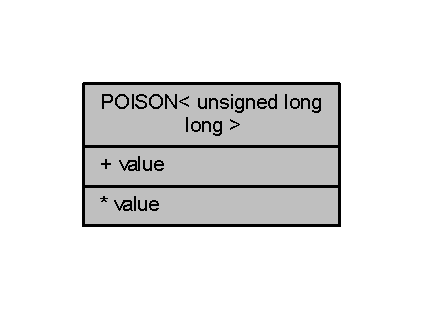
\includegraphics[width=203pt]{struct_p_o_i_s_o_n_3_01unsigned_01long_01long_01_4__coll__graph}
\end{center}
\end{figure}
\subsection*{Static Public Attributes}
\textbf{ }\par
\begin{DoxyCompactItemize}
\item 
\mbox{\Hypertarget{struct_p_o_i_s_o_n_3_01unsigned_01long_01long_01_4_aaeb0e299161215b97c3121c6374c5d24}\label{struct_p_o_i_s_o_n_3_01unsigned_01long_01long_01_4_aaeb0e299161215b97c3121c6374c5d24}} 
static const unsigned long long {\bfseries value} = 147520069954\+U\+LL
\end{DoxyCompactItemize}



The documentation for this struct was generated from the following file\+:\begin{DoxyCompactItemize}
\item 
D\+:/\+Git\+Hub/\+Techno\+Atom/src/\hyperlink{debug__tools_8h}{debug\+\_\+tools.\+h}\end{DoxyCompactItemize}

\hypertarget{struct_p_o_i_s_o_n_3_01unsigned_01short_01_4}{}\section{P\+O\+I\+S\+ON$<$ unsigned short $>$ Struct Template Reference}
\label{struct_p_o_i_s_o_n_3_01unsigned_01short_01_4}\index{P\+O\+I\+S\+O\+N$<$ unsigned short $>$@{P\+O\+I\+S\+O\+N$<$ unsigned short $>$}}


Collaboration diagram for P\+O\+I\+S\+ON$<$ unsigned short $>$\+:
\nopagebreak
\begin{figure}[H]
\begin{center}
\leavevmode
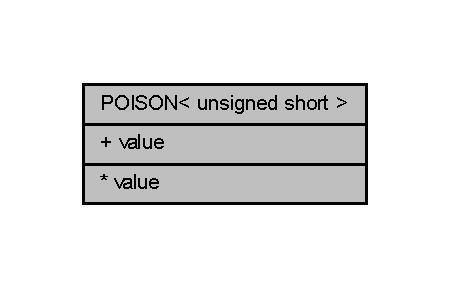
\includegraphics[width=216pt]{struct_p_o_i_s_o_n_3_01unsigned_01short_01_4__coll__graph}
\end{center}
\end{figure}
\subsection*{Static Public Attributes}
\textbf{ }\par
\begin{DoxyCompactItemize}
\item 
\mbox{\Hypertarget{struct_p_o_i_s_o_n_3_01unsigned_01short_01_4_a0a82e6d7b747a1a3eeeafa834ae87029}\label{struct_p_o_i_s_o_n_3_01unsigned_01short_01_4_a0a82e6d7b747a1a3eeeafa834ae87029}} 
static const unsigned short {\bfseries value} = 121
\end{DoxyCompactItemize}



The documentation for this struct was generated from the following file\+:\begin{DoxyCompactItemize}
\item 
D\+:/\+Git\+Hub/\+Techno\+Atom/src/\hyperlink{debug__tools_8h}{debug\+\_\+tools.\+h}\end{DoxyCompactItemize}

\hypertarget{classatom_1_1stack__t}{}\section{atom\+:\+:stack\+\_\+t$<$ Tp, Container $>$ Class Template Reference}
\label{classatom_1_1stack__t}\index{atom\+::stack\+\_\+t$<$ Tp, Container $>$@{atom\+::stack\+\_\+t$<$ Tp, Container $>$}}


{\ttfamily \#include $<$stack.\+h$>$}



Collaboration diagram for atom\+:\+:stack\+\_\+t$<$ Tp, Container $>$\+:
\nopagebreak
\begin{figure}[H]
\begin{center}
\leavevmode
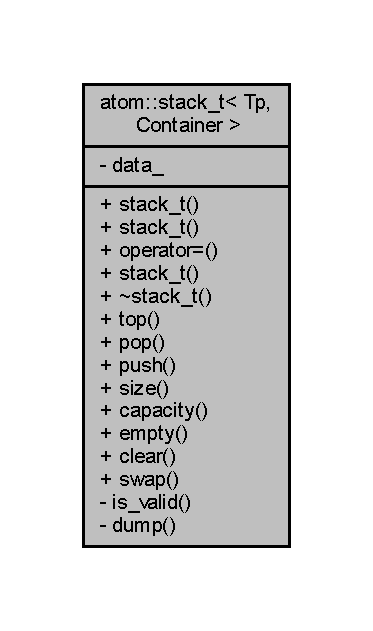
\includegraphics[width=179pt]{classatom_1_1stack__t__coll__graph}
\end{center}
\end{figure}
\subsection*{Public Types}
\begin{DoxyCompactItemize}
\item 
\mbox{\Hypertarget{classatom_1_1stack__t_a37733753643a75fca01979480f888d8e}\label{classatom_1_1stack__t_a37733753643a75fca01979480f888d8e}} 
using \hyperlink{classatom_1_1stack__t_a37733753643a75fca01979480f888d8e}{value\+\_\+type} = typename Container\+::value\+\_\+type
\begin{DoxyCompactList}\small\item\em Element type. \end{DoxyCompactList}\item 
\mbox{\Hypertarget{classatom_1_1stack__t_a780222269dc9f9323438ec4c56795735}\label{classatom_1_1stack__t_a780222269dc9f9323438ec4c56795735}} 
using \hyperlink{classatom_1_1stack__t_a780222269dc9f9323438ec4c56795735}{const\+\_\+value\+\_\+type} = typename Container\+::const\+\_\+value\+\_\+type
\begin{DoxyCompactList}\small\item\em Const element type. \end{DoxyCompactList}\item 
\mbox{\Hypertarget{classatom_1_1stack__t_a43888b80c0b6cceea0509a3646823f98}\label{classatom_1_1stack__t_a43888b80c0b6cceea0509a3646823f98}} 
using \hyperlink{classatom_1_1stack__t_a43888b80c0b6cceea0509a3646823f98}{size\+\_\+type} = typename Container\+::size\+\_\+type
\begin{DoxyCompactList}\small\item\em Size type. \end{DoxyCompactList}\item 
\mbox{\Hypertarget{classatom_1_1stack__t_ab18a4ad6c754ddb70ce585528823eac2}\label{classatom_1_1stack__t_ab18a4ad6c754ddb70ce585528823eac2}} 
using \hyperlink{classatom_1_1stack__t_ab18a4ad6c754ddb70ce585528823eac2}{container\+\_\+type} = Container
\begin{DoxyCompactList}\small\item\em Type of the container. \end{DoxyCompactList}\end{DoxyCompactItemize}
\subsection*{Public Member Functions}
\begin{DoxyCompactItemize}
\item 
\mbox{\Hypertarget{classatom_1_1stack__t_a03f4e7718f28fc1e62e70ad202f21d90}\label{classatom_1_1stack__t_a03f4e7718f28fc1e62e70ad202f21d90}} 
\hyperlink{classatom_1_1stack__t_a03f4e7718f28fc1e62e70ad202f21d90}{stack\+\_\+t} ()=default
\begin{DoxyCompactList}\small\item\em Default constructor. \end{DoxyCompactList}\item 
\hyperlink{classatom_1_1stack__t_a519cc745d74f25e1e73168d63bd7ce4a}{stack\+\_\+t} (const \hyperlink{classatom_1_1stack__t}{stack\+\_\+t} \&that)
\begin{DoxyCompactList}\small\item\em The copy constructor. \end{DoxyCompactList}\item 
const \hyperlink{classatom_1_1stack__t}{stack\+\_\+t} \& \hyperlink{classatom_1_1stack__t_a9b0f89271398f910e88a88014f29669d}{operator=} (const \hyperlink{classatom_1_1stack__t}{stack\+\_\+t} \&that)
\begin{DoxyCompactList}\small\item\em The assignment operator. \end{DoxyCompactList}\item 
\hyperlink{classatom_1_1stack__t_a2423a055415e15266b1625ad78b38baf}{stack\+\_\+t} (const \hyperlink{classatom_1_1stack__t}{stack\+\_\+t} \&\&that) noexcept
\begin{DoxyCompactList}\small\item\em The move constructor. \end{DoxyCompactList}\item 
\mbox{\Hypertarget{classatom_1_1stack__t_a08decda2a6cd788029c0d6b58b8d20b9}\label{classatom_1_1stack__t_a08decda2a6cd788029c0d6b58b8d20b9}} 
\hyperlink{classatom_1_1stack__t_a08decda2a6cd788029c0d6b58b8d20b9}{$\sim$stack\+\_\+t} ()=default
\begin{DoxyCompactList}\small\item\em Destructor. \end{DoxyCompactList}\item 
\hyperlink{classatom_1_1stack__t_a37733753643a75fca01979480f888d8e}{value\+\_\+type} \hyperlink{classatom_1_1stack__t_a80818d88b68e425c679abbfda849c005}{top} () const
\begin{DoxyCompactList}\small\item\em Get the item from the stack. \end{DoxyCompactList}\item 
void \hyperlink{classatom_1_1stack__t_a86b9e880776b1ee326d07dee157c4991}{pop} ()
\begin{DoxyCompactList}\small\item\em Delete the item from the stack. \end{DoxyCompactList}\item 
void \hyperlink{classatom_1_1stack__t_aebddf7b02c7317f9edc25741412fccb7}{push} (\hyperlink{classatom_1_1stack__t_a780222269dc9f9323438ec4c56795735}{const\+\_\+value\+\_\+type} \&x)
\begin{DoxyCompactList}\small\item\em Append new item in the stack. \end{DoxyCompactList}\item 
\hyperlink{classatom_1_1stack__t_a43888b80c0b6cceea0509a3646823f98}{size\+\_\+type} \hyperlink{classatom_1_1stack__t_a7ae2d64181c0dcc03a54ca5df4c0de75}{size} () const noexcept
\begin{DoxyCompactList}\small\item\em Currently size of the stack. \end{DoxyCompactList}\item 
\hyperlink{classatom_1_1stack__t_a43888b80c0b6cceea0509a3646823f98}{size\+\_\+type} \hyperlink{classatom_1_1stack__t_ace44f2ab1b95b156fd30e25f26f8065e}{capacity} () const noexcept
\begin{DoxyCompactList}\small\item\em Capacity. \end{DoxyCompactList}\item 
bool \hyperlink{classatom_1_1stack__t_a3db873b3a1217f10fc1d6154d717b84d}{empty} () const noexcept
\begin{DoxyCompactList}\small\item\em Checks the emptiness of the stack. \end{DoxyCompactList}\item 
\mbox{\Hypertarget{classatom_1_1stack__t_a2f631f7283574b82b0776c740a13d41a}\label{classatom_1_1stack__t_a2f631f7283574b82b0776c740a13d41a}} 
void \hyperlink{classatom_1_1stack__t_a2f631f7283574b82b0776c740a13d41a}{clear} () const noexcept
\begin{DoxyCompactList}\small\item\em Clear the stack. \end{DoxyCompactList}\item 
void \hyperlink{classatom_1_1stack__t_a05922491d108df9aeae30a5da18d7192}{swap} (\hyperlink{classatom_1_1stack__t}{stack\+\_\+t} \&rhs) noexcept
\begin{DoxyCompactList}\small\item\em swap two stack \end{DoxyCompactList}\end{DoxyCompactItemize}
\subsection*{Private Member Functions}
\begin{DoxyCompactItemize}
\item 
bool \hyperlink{classatom_1_1stack__t_aad558411c92e7c1776ad82be0ea876ee}{is\+\_\+valid} () const noexcept
\begin{DoxyCompactList}\small\item\em Silent verifier. \end{DoxyCompactList}\item 
void \hyperlink{classatom_1_1stack__t_a424f65300ba04f8000ec6bf315595d1b}{dump} (const char $\ast$function\+\_\+name, int line\+\_\+number) const noexcept
\begin{DoxyCompactList}\small\item\em Dumper. \end{DoxyCompactList}\end{DoxyCompactItemize}
\subsection*{Private Attributes}
\begin{DoxyCompactItemize}
\item 
\mbox{\Hypertarget{classatom_1_1stack__t_a5c58ed4bf4abd24da5d98f28f085dff6}\label{classatom_1_1stack__t_a5c58ed4bf4abd24da5d98f28f085dff6}} 
\hyperlink{classatom_1_1stack__t_ab18a4ad6c754ddb70ce585528823eac2}{container\+\_\+type} \hyperlink{classatom_1_1stack__t_a5c58ed4bf4abd24da5d98f28f085dff6}{data\+\_\+}
\begin{DoxyCompactList}\small\item\em Container, base of the stack. \end{DoxyCompactList}\end{DoxyCompactItemize}


\subsection{Detailed Description}
\subsubsection*{template$<$typename Tp, typename Container = atom\+::vector\+\_\+t$<$\+Tp$>$$>$\newline
class atom\+::stack\+\_\+t$<$ Tp, Container $>$}


\begin{DoxyTemplParams}{Template Parameters}
{\em Tp} & The type of the value in the stack \\
\hline
{\em Container} & the type of container which houses the stack (default is \hyperlink{classatom_1_1vector__t}{atom\+::vector\+\_\+t})\\
\hline
\end{DoxyTemplParams}
Container must have function\+: push\+\_\+back(), erase(), back(), \hyperlink{classatom_1_1stack__t_a7ae2d64181c0dcc03a54ca5df4c0de75}{size()}, \hyperlink{classatom_1_1stack__t_a05922491d108df9aeae30a5da18d7192}{swap()} and \hyperlink{classatom_1_1stack__t_ace44f2ab1b95b156fd30e25f26f8065e}{capacity()} 

\subsection{Constructor \& Destructor Documentation}
\mbox{\Hypertarget{classatom_1_1stack__t_a519cc745d74f25e1e73168d63bd7ce4a}\label{classatom_1_1stack__t_a519cc745d74f25e1e73168d63bd7ce4a}} 
\index{atom\+::stack\+\_\+t@{atom\+::stack\+\_\+t}!stack\+\_\+t@{stack\+\_\+t}}
\index{stack\+\_\+t@{stack\+\_\+t}!atom\+::stack\+\_\+t@{atom\+::stack\+\_\+t}}
\subsubsection{\texorpdfstring{stack\+\_\+t()}{stack\_t()}\hspace{0.1cm}{\footnotesize\ttfamily [1/2]}}
{\footnotesize\ttfamily template$<$typename Tp , typename Container  = atom\+::vector\+\_\+t$<$\+Tp$>$$>$ \\
\hyperlink{classatom_1_1stack__t}{atom\+::stack\+\_\+t}$<$ Tp, Container $>$\+::\hyperlink{classatom_1_1stack__t}{stack\+\_\+t} (\begin{DoxyParamCaption}\item[{const \hyperlink{classatom_1_1stack__t}{stack\+\_\+t}$<$ Tp, Container $>$ \&}]{that }\end{DoxyParamCaption})\hspace{0.3cm}{\ttfamily [inline]}}



The copy constructor. 


\begin{DoxyParams}{Parameters}
{\em that} & The copy source \\
\hline
\end{DoxyParams}
\mbox{\Hypertarget{classatom_1_1stack__t_a2423a055415e15266b1625ad78b38baf}\label{classatom_1_1stack__t_a2423a055415e15266b1625ad78b38baf}} 
\index{atom\+::stack\+\_\+t@{atom\+::stack\+\_\+t}!stack\+\_\+t@{stack\+\_\+t}}
\index{stack\+\_\+t@{stack\+\_\+t}!atom\+::stack\+\_\+t@{atom\+::stack\+\_\+t}}
\subsubsection{\texorpdfstring{stack\+\_\+t()}{stack\_t()}\hspace{0.1cm}{\footnotesize\ttfamily [2/2]}}
{\footnotesize\ttfamily template$<$typename Tp , typename Container  = atom\+::vector\+\_\+t$<$\+Tp$>$$>$ \\
\hyperlink{classatom_1_1stack__t}{atom\+::stack\+\_\+t}$<$ Tp, Container $>$\+::\hyperlink{classatom_1_1stack__t}{stack\+\_\+t} (\begin{DoxyParamCaption}\item[{const \hyperlink{classatom_1_1stack__t}{stack\+\_\+t}$<$ Tp, Container $>$ \&\&}]{that }\end{DoxyParamCaption})\hspace{0.3cm}{\ttfamily [inline]}, {\ttfamily [noexcept]}}



The move constructor. 


\begin{DoxyParams}{Parameters}
{\em that} & The move source \\
\hline
\end{DoxyParams}


\subsection{Member Function Documentation}
\mbox{\Hypertarget{classatom_1_1stack__t_ace44f2ab1b95b156fd30e25f26f8065e}\label{classatom_1_1stack__t_ace44f2ab1b95b156fd30e25f26f8065e}} 
\index{atom\+::stack\+\_\+t@{atom\+::stack\+\_\+t}!capacity@{capacity}}
\index{capacity@{capacity}!atom\+::stack\+\_\+t@{atom\+::stack\+\_\+t}}
\subsubsection{\texorpdfstring{capacity()}{capacity()}}
{\footnotesize\ttfamily template$<$typename Tp , typename Container  = atom\+::vector\+\_\+t$<$\+Tp$>$$>$ \\
\hyperlink{classatom_1_1stack__t_a43888b80c0b6cceea0509a3646823f98}{size\+\_\+type} \hyperlink{classatom_1_1stack__t}{atom\+::stack\+\_\+t}$<$ Tp, Container $>$\+::capacity (\begin{DoxyParamCaption}{ }\end{DoxyParamCaption}) const\hspace{0.3cm}{\ttfamily [inline]}, {\ttfamily [noexcept]}}



Capacity. 

\begin{DoxyReturn}{Returns}
Capacity of the stack 
\end{DoxyReturn}
\mbox{\Hypertarget{classatom_1_1stack__t_a424f65300ba04f8000ec6bf315595d1b}\label{classatom_1_1stack__t_a424f65300ba04f8000ec6bf315595d1b}} 
\index{atom\+::stack\+\_\+t@{atom\+::stack\+\_\+t}!dump@{dump}}
\index{dump@{dump}!atom\+::stack\+\_\+t@{atom\+::stack\+\_\+t}}
\subsubsection{\texorpdfstring{dump()}{dump()}}
{\footnotesize\ttfamily template$<$typename Tp , typename Container $>$ \\
void \hyperlink{classatom_1_1stack__t}{atom\+::stack\+\_\+t}$<$ Tp, Container $>$\+::dump (\begin{DoxyParamCaption}\item[{const char $\ast$}]{function\+\_\+name,  }\item[{int}]{line\+\_\+number }\end{DoxyParamCaption}) const\hspace{0.3cm}{\ttfamily [private]}, {\ttfamily [noexcept]}}



Dumper. 

Create file \char`\"{}\+\_\+\+\_\+stack\+\_\+dump.\+txt\char`\"{} where is information about stack\textquotesingle{}s status

Macro A\+T\+O\+M\+\_\+\+N\+W\+R\+I\+TE prohibit function \hyperlink{classatom_1_1stack__t_a424f65300ba04f8000ec6bf315595d1b}{dump()} print elements (for example when value\+\_\+type has not operator$<$$<$) 
\begin{DoxyParams}{Parameters}
{\em function\+\_\+name} & Name of function which call this method \\
\hline
{\em line\+\_\+number} & Number of the line where call this method \\
\hline
\end{DoxyParams}
\mbox{\Hypertarget{classatom_1_1stack__t_a3db873b3a1217f10fc1d6154d717b84d}\label{classatom_1_1stack__t_a3db873b3a1217f10fc1d6154d717b84d}} 
\index{atom\+::stack\+\_\+t@{atom\+::stack\+\_\+t}!empty@{empty}}
\index{empty@{empty}!atom\+::stack\+\_\+t@{atom\+::stack\+\_\+t}}
\subsubsection{\texorpdfstring{empty()}{empty()}}
{\footnotesize\ttfamily template$<$typename Tp , typename Container  = atom\+::vector\+\_\+t$<$\+Tp$>$$>$ \\
bool \hyperlink{classatom_1_1stack__t}{atom\+::stack\+\_\+t}$<$ Tp, Container $>$\+::empty (\begin{DoxyParamCaption}{ }\end{DoxyParamCaption}) const\hspace{0.3cm}{\ttfamily [inline]}, {\ttfamily [noexcept]}}



Checks the emptiness of the stack. 

\begin{DoxyReturn}{Returns}
True if stack is empty, otherwise false 
\end{DoxyReturn}
\mbox{\Hypertarget{classatom_1_1stack__t_aad558411c92e7c1776ad82be0ea876ee}\label{classatom_1_1stack__t_aad558411c92e7c1776ad82be0ea876ee}} 
\index{atom\+::stack\+\_\+t@{atom\+::stack\+\_\+t}!is\+\_\+valid@{is\+\_\+valid}}
\index{is\+\_\+valid@{is\+\_\+valid}!atom\+::stack\+\_\+t@{atom\+::stack\+\_\+t}}
\subsubsection{\texorpdfstring{is\+\_\+valid()}{is\_valid()}}
{\footnotesize\ttfamily template$<$typename Tp , typename Container  = atom\+::vector\+\_\+t$<$\+Tp$>$$>$ \\
bool \hyperlink{classatom_1_1stack__t}{atom\+::stack\+\_\+t}$<$ Tp, Container $>$\+::is\+\_\+valid (\begin{DoxyParamCaption}{ }\end{DoxyParamCaption}) const\hspace{0.3cm}{\ttfamily [inline]}, {\ttfamily [private]}, {\ttfamily [noexcept]}}



Silent verifier. 

\begin{DoxyReturn}{Returns}
True if stack is valid else return false 
\end{DoxyReturn}
\mbox{\Hypertarget{classatom_1_1stack__t_a9b0f89271398f910e88a88014f29669d}\label{classatom_1_1stack__t_a9b0f89271398f910e88a88014f29669d}} 
\index{atom\+::stack\+\_\+t@{atom\+::stack\+\_\+t}!operator=@{operator=}}
\index{operator=@{operator=}!atom\+::stack\+\_\+t@{atom\+::stack\+\_\+t}}
\subsubsection{\texorpdfstring{operator=()}{operator=()}}
{\footnotesize\ttfamily template$<$typename Tp , typename Container  = atom\+::vector\+\_\+t$<$\+Tp$>$$>$ \\
const \hyperlink{classatom_1_1stack__t}{stack\+\_\+t}\& \hyperlink{classatom_1_1stack__t}{atom\+::stack\+\_\+t}$<$ Tp, Container $>$\+::operator= (\begin{DoxyParamCaption}\item[{const \hyperlink{classatom_1_1stack__t}{stack\+\_\+t}$<$ Tp, Container $>$ \&}]{that }\end{DoxyParamCaption})\hspace{0.3cm}{\ttfamily [inline]}}



The assignment operator. 

Use copy and move idiom 
\begin{DoxyParams}{Parameters}
{\em that} & The source of the assignment \\
\hline
\end{DoxyParams}

\begin{DoxyExceptions}{Exceptions}
{\em The} & same exceptions as the \hyperlink{classatom_1_1stack__t_a519cc745d74f25e1e73168d63bd7ce4a}{stack\+\_\+t(const stack\+\_\+t\&)} \\
\hline
\end{DoxyExceptions}
\begin{DoxyReturn}{Returns}
Constant reference to the calling object 
\end{DoxyReturn}
\mbox{\Hypertarget{classatom_1_1stack__t_a86b9e880776b1ee326d07dee157c4991}\label{classatom_1_1stack__t_a86b9e880776b1ee326d07dee157c4991}} 
\index{atom\+::stack\+\_\+t@{atom\+::stack\+\_\+t}!pop@{pop}}
\index{pop@{pop}!atom\+::stack\+\_\+t@{atom\+::stack\+\_\+t}}
\subsubsection{\texorpdfstring{pop()}{pop()}}
{\footnotesize\ttfamily template$<$typename Tp , typename Container  = atom\+::vector\+\_\+t$<$\+Tp$>$$>$ \\
void \hyperlink{classatom_1_1stack__t}{atom\+::stack\+\_\+t}$<$ Tp, Container $>$\+::pop (\begin{DoxyParamCaption}{ }\end{DoxyParamCaption})\hspace{0.3cm}{\ttfamily [inline]}}



Delete the item from the stack. 

If stack is empty does nothing 
\begin{DoxyExceptions}{Exceptions}
{\em \hyperlink{classatom_1_1invalid_object}{atom\+::invalid\+Object}} & From \hyperlink{debug__tools_8h_a273b49426c51bc6a7eb989ee0acbdc6b}{A\+T\+O\+M\+\_\+\+A\+S\+S\+E\+R\+T\+\_\+\+V\+A\+L\+I\+D()} when stack is not valid \\
\hline
\end{DoxyExceptions}
\mbox{\Hypertarget{classatom_1_1stack__t_aebddf7b02c7317f9edc25741412fccb7}\label{classatom_1_1stack__t_aebddf7b02c7317f9edc25741412fccb7}} 
\index{atom\+::stack\+\_\+t@{atom\+::stack\+\_\+t}!push@{push}}
\index{push@{push}!atom\+::stack\+\_\+t@{atom\+::stack\+\_\+t}}
\subsubsection{\texorpdfstring{push()}{push()}}
{\footnotesize\ttfamily template$<$typename Tp , typename Container  = atom\+::vector\+\_\+t$<$\+Tp$>$$>$ \\
void \hyperlink{classatom_1_1stack__t}{atom\+::stack\+\_\+t}$<$ Tp, Container $>$\+::push (\begin{DoxyParamCaption}\item[{\hyperlink{classatom_1_1stack__t_a780222269dc9f9323438ec4c56795735}{const\+\_\+value\+\_\+type} \&}]{x }\end{DoxyParamCaption})\hspace{0.3cm}{\ttfamily [inline]}}



Append new item in the stack. 


\begin{DoxyParams}{Parameters}
{\em x} & The element that will be added to the stack \\
\hline
\end{DoxyParams}

\begin{DoxyExceptions}{Exceptions}
{\em \hyperlink{classatom_1_1invalid_object}{atom\+::invalid\+Object}} & From \hyperlink{debug__tools_8h_a273b49426c51bc6a7eb989ee0acbdc6b}{A\+T\+O\+M\+\_\+\+A\+S\+S\+E\+R\+T\+\_\+\+V\+A\+L\+I\+D()} when stack is not valid \\
\hline
{\em The} & same exceptions as the function push\+\_\+back() (from container) \\
\hline
\end{DoxyExceptions}
\mbox{\Hypertarget{classatom_1_1stack__t_a7ae2d64181c0dcc03a54ca5df4c0de75}\label{classatom_1_1stack__t_a7ae2d64181c0dcc03a54ca5df4c0de75}} 
\index{atom\+::stack\+\_\+t@{atom\+::stack\+\_\+t}!size@{size}}
\index{size@{size}!atom\+::stack\+\_\+t@{atom\+::stack\+\_\+t}}
\subsubsection{\texorpdfstring{size()}{size()}}
{\footnotesize\ttfamily template$<$typename Tp , typename Container  = atom\+::vector\+\_\+t$<$\+Tp$>$$>$ \\
\hyperlink{classatom_1_1stack__t_a43888b80c0b6cceea0509a3646823f98}{size\+\_\+type} \hyperlink{classatom_1_1stack__t}{atom\+::stack\+\_\+t}$<$ Tp, Container $>$\+::size (\begin{DoxyParamCaption}{ }\end{DoxyParamCaption}) const\hspace{0.3cm}{\ttfamily [inline]}, {\ttfamily [noexcept]}}



Currently size of the stack. 

\begin{DoxyReturn}{Returns}
Count of the item in the stack 
\end{DoxyReturn}
\mbox{\Hypertarget{classatom_1_1stack__t_a05922491d108df9aeae30a5da18d7192}\label{classatom_1_1stack__t_a05922491d108df9aeae30a5da18d7192}} 
\index{atom\+::stack\+\_\+t@{atom\+::stack\+\_\+t}!swap@{swap}}
\index{swap@{swap}!atom\+::stack\+\_\+t@{atom\+::stack\+\_\+t}}
\subsubsection{\texorpdfstring{swap()}{swap()}}
{\footnotesize\ttfamily template$<$typename Tp , typename Container  = atom\+::vector\+\_\+t$<$\+Tp$>$$>$ \\
void \hyperlink{classatom_1_1stack__t}{atom\+::stack\+\_\+t}$<$ Tp, Container $>$\+::swap (\begin{DoxyParamCaption}\item[{\hyperlink{classatom_1_1stack__t}{stack\+\_\+t}$<$ Tp, Container $>$ \&}]{rhs }\end{DoxyParamCaption})\hspace{0.3cm}{\ttfamily [inline]}, {\ttfamily [noexcept]}}



swap two stack 


\begin{DoxyParams}{Parameters}
{\em rhs} & other stack to which you want to exchange \\
\hline
\end{DoxyParams}
\mbox{\Hypertarget{classatom_1_1stack__t_a80818d88b68e425c679abbfda849c005}\label{classatom_1_1stack__t_a80818d88b68e425c679abbfda849c005}} 
\index{atom\+::stack\+\_\+t@{atom\+::stack\+\_\+t}!top@{top}}
\index{top@{top}!atom\+::stack\+\_\+t@{atom\+::stack\+\_\+t}}
\subsubsection{\texorpdfstring{top()}{top()}}
{\footnotesize\ttfamily template$<$typename Tp , typename Container  = atom\+::vector\+\_\+t$<$\+Tp$>$$>$ \\
\hyperlink{classatom_1_1stack__t_a37733753643a75fca01979480f888d8e}{value\+\_\+type} \hyperlink{classatom_1_1stack__t}{atom\+::stack\+\_\+t}$<$ Tp, Container $>$\+::top (\begin{DoxyParamCaption}{ }\end{DoxyParamCaption}) const\hspace{0.3cm}{\ttfamily [inline]}}



Get the item from the stack. 


\begin{DoxyExceptions}{Exceptions}
{\em The} & same exceptions as the function back() (from container) \\
\hline
\end{DoxyExceptions}
\begin{DoxyReturn}{Returns}
The top item from the stack 
\end{DoxyReturn}


The documentation for this class was generated from the following files\+:\begin{DoxyCompactItemize}
\item 
D\+:/\+Git\+Hub/\+Techno\+Atom/task 2/src/stack/\hyperlink{stack_8h}{stack.\+h}\item 
D\+:/\+Git\+Hub/\+Techno\+Atom/task 2/src/stack/implement/stack.\+hpp\end{DoxyCompactItemize}

\hypertarget{classatom_1_1vector__t}{}\section{atom\+:\+:vector\+\_\+t$<$ Tp $>$ Class Template Reference}
\label{classatom_1_1vector__t}\index{atom\+::vector\+\_\+t$<$ Tp $>$@{atom\+::vector\+\_\+t$<$ Tp $>$}}


{\ttfamily \#include $<$vector.\+h$>$}



Collaboration diagram for atom\+:\+:vector\+\_\+t$<$ Tp $>$\+:
\nopagebreak
\begin{figure}[H]
\begin{center}
\leavevmode
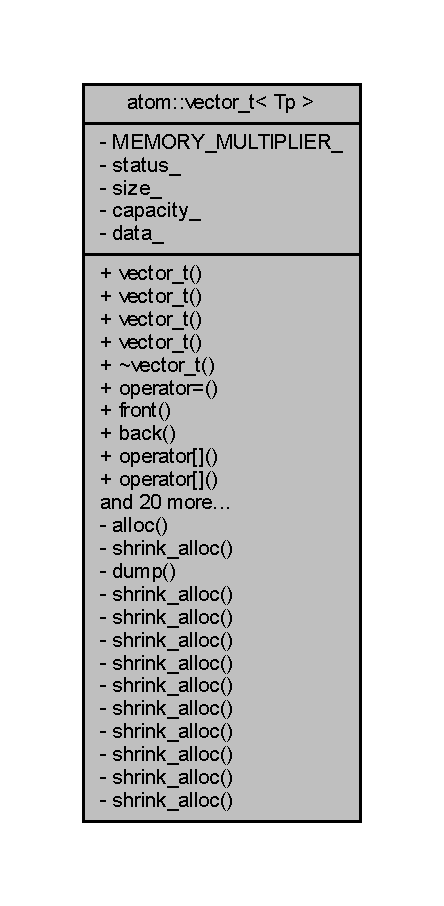
\includegraphics[width=213pt]{classatom_1_1vector__t__coll__graph}
\end{center}
\end{figure}
\subsection*{Public Types}
\begin{DoxyCompactItemize}
\item 
\mbox{\Hypertarget{classatom_1_1vector__t_a558283a4fed53856d445ceb61ac96d94}\label{classatom_1_1vector__t_a558283a4fed53856d445ceb61ac96d94}} 
using \hyperlink{classatom_1_1vector__t_a558283a4fed53856d445ceb61ac96d94}{value\+\_\+type} = Tp
\begin{DoxyCompactList}\small\item\em Element type. \end{DoxyCompactList}\item 
\mbox{\Hypertarget{classatom_1_1vector__t_a14fe7ee127e522f41f345462311c924e}\label{classatom_1_1vector__t_a14fe7ee127e522f41f345462311c924e}} 
using \hyperlink{classatom_1_1vector__t_a14fe7ee127e522f41f345462311c924e}{const\+\_\+value\+\_\+type} = const Tp
\begin{DoxyCompactList}\small\item\em Const element type. \end{DoxyCompactList}\item 
\mbox{\Hypertarget{classatom_1_1vector__t_a1790d79321f4fa8d2580474dd0f56033}\label{classatom_1_1vector__t_a1790d79321f4fa8d2580474dd0f56033}} 
using \hyperlink{classatom_1_1vector__t_a1790d79321f4fa8d2580474dd0f56033}{size\+\_\+type} = std\+::size\+\_\+t
\begin{DoxyCompactList}\small\item\em Size type. \end{DoxyCompactList}\end{DoxyCompactItemize}
\subsection*{Public Member Functions}
\begin{DoxyCompactItemize}
\item 
\mbox{\Hypertarget{classatom_1_1vector__t_a72425f7c04f5d5fffd5244596c9a33c0}\label{classatom_1_1vector__t_a72425f7c04f5d5fffd5244596c9a33c0}} 
\hyperlink{classatom_1_1vector__t_a72425f7c04f5d5fffd5244596c9a33c0}{vector\+\_\+t} () noexcept
\begin{DoxyCompactList}\small\item\em Default constructor. \end{DoxyCompactList}\item 
\hyperlink{classatom_1_1vector__t_a6c045495ebfcd53b4d91d9c76ceb5fdf}{vector\+\_\+t} (const \hyperlink{classatom_1_1vector__t_a1790d79321f4fa8d2580474dd0f56033}{size\+\_\+type} n, const \hyperlink{classatom_1_1vector__t_a558283a4fed53856d445ceb61ac96d94}{value\+\_\+type} \&value=\hyperlink{classatom_1_1vector__t_a558283a4fed53856d445ceb61ac96d94}{value\+\_\+type}())
\begin{DoxyCompactList}\small\item\em Constructor. \end{DoxyCompactList}\item 
\hyperlink{classatom_1_1vector__t_a2c546a0310265fa1eabcc21ac4349d33}{vector\+\_\+t} (const \hyperlink{classatom_1_1vector__t}{vector\+\_\+t} \&that)
\begin{DoxyCompactList}\small\item\em The copy constructor. \end{DoxyCompactList}\item 
\hyperlink{classatom_1_1vector__t_a7fb03f8164c86f7e9df312fe4da33fd0}{vector\+\_\+t} (\hyperlink{classatom_1_1vector__t}{vector\+\_\+t} \&\&that) noexcept
\begin{DoxyCompactList}\small\item\em The move constructor. \end{DoxyCompactList}\item 
\hyperlink{classatom_1_1vector__t_afa9985af7e737691bfd4fc2c876c3378}{$\sim$vector\+\_\+t} ()
\begin{DoxyCompactList}\small\item\em Destructor. \end{DoxyCompactList}\item 
const \hyperlink{classatom_1_1vector__t}{vector\+\_\+t} \& \hyperlink{classatom_1_1vector__t_af0b2037e8034d5bb97ac320f4513df2d}{operator=} (const \hyperlink{classatom_1_1vector__t}{vector\+\_\+t} \&that)
\begin{DoxyCompactList}\small\item\em The assignment operator. \end{DoxyCompactList}\item 
\hyperlink{classatom_1_1vector__t_a14fe7ee127e522f41f345462311c924e}{const\+\_\+value\+\_\+type} \& \hyperlink{classatom_1_1vector__t_a1c0df3e4399ea92d4213986c2e5359bf}{front} () const
\begin{DoxyCompactList}\small\item\em First element. \end{DoxyCompactList}\item 
\hyperlink{classatom_1_1vector__t_a14fe7ee127e522f41f345462311c924e}{const\+\_\+value\+\_\+type} \& \hyperlink{classatom_1_1vector__t_a081ce30b6b112520ce41879cf383a409}{back} () const
\begin{DoxyCompactList}\small\item\em Last element. \end{DoxyCompactList}\item 
\hyperlink{classatom_1_1vector__t_a558283a4fed53856d445ceb61ac96d94}{value\+\_\+type} \& \hyperlink{classatom_1_1vector__t_aa8d100ece074c429aafe4cd110165643}{operator\mbox{[}$\,$\mbox{]}} (const \hyperlink{classatom_1_1vector__t_a1790d79321f4fa8d2580474dd0f56033}{size\+\_\+type} n)
\begin{DoxyCompactList}\small\item\em Operator addressing. \end{DoxyCompactList}\item 
\hyperlink{classatom_1_1vector__t_a14fe7ee127e522f41f345462311c924e}{const\+\_\+value\+\_\+type} \& \hyperlink{classatom_1_1vector__t_ab3cbcfdd1fdadcd927eb1ef629d2f814}{operator\mbox{[}$\,$\mbox{]}} (const \hyperlink{classatom_1_1vector__t_a1790d79321f4fa8d2580474dd0f56033}{size\+\_\+type} n) const
\begin{DoxyCompactList}\small\item\em Operator addressing. \end{DoxyCompactList}\item 
void \hyperlink{classatom_1_1vector__t_a92c657f98ab473119a6b04dad7cd2091}{push\+\_\+back} (\hyperlink{classatom_1_1vector__t_a14fe7ee127e522f41f345462311c924e}{const\+\_\+value\+\_\+type} x)
\begin{DoxyCompactList}\small\item\em Push new item in back of the vector. \end{DoxyCompactList}\item 
bool \hyperlink{classatom_1_1vector__t_ab414b36ee5235f86352dbdb73ff6c0e0}{erase} (const \hyperlink{classatom_1_1vector__t_a1790d79321f4fa8d2580474dd0f56033}{size\+\_\+type} position)
\begin{DoxyCompactList}\small\item\em Remove nth element. \end{DoxyCompactList}\item 
\mbox{\Hypertarget{classatom_1_1vector__t_a6a6e6950a03b50dd330c2b54f8a6104a}\label{classatom_1_1vector__t_a6a6e6950a03b50dd330c2b54f8a6104a}} 
void \hyperlink{classatom_1_1vector__t_a6a6e6950a03b50dd330c2b54f8a6104a}{clear} () noexcept
\begin{DoxyCompactList}\small\item\em Clear the vector. \end{DoxyCompactList}\item 
void \hyperlink{classatom_1_1vector__t_a76f6cab17dbffe1a54657199b6a5cb55}{reserve} (const \hyperlink{classatom_1_1vector__t_a1790d79321f4fa8d2580474dd0f56033}{size\+\_\+type} n)
\begin{DoxyCompactList}\small\item\em Reserve new memory. \end{DoxyCompactList}\item 
void \hyperlink{classatom_1_1vector__t_a5720e4e26657a55697d4335663cb6f10}{resize} (const \hyperlink{classatom_1_1vector__t_a1790d79321f4fa8d2580474dd0f56033}{size\+\_\+type} n, const \hyperlink{classatom_1_1vector__t_a558283a4fed53856d445ceb61ac96d94}{value\+\_\+type} \&value=\hyperlink{classatom_1_1vector__t_a558283a4fed53856d445ceb61ac96d94}{value\+\_\+type}())
\begin{DoxyCompactList}\small\item\em Create new block of the memory. \end{DoxyCompactList}\item 
bool \hyperlink{classatom_1_1vector__t_a0204758afeafe695689a8c926fa79897}{empty} () const noexcept
\begin{DoxyCompactList}\small\item\em Checks the vector on the void. \end{DoxyCompactList}\item 
\hyperlink{classatom_1_1vector__t_a1790d79321f4fa8d2580474dd0f56033}{size\+\_\+type} \hyperlink{classatom_1_1vector__t_ada6d9f1b78bbb338980c4bd714cd3096}{capacity} () const noexcept
\begin{DoxyCompactList}\small\item\em Capacity. \end{DoxyCompactList}\item 
\hyperlink{classatom_1_1vector__t_a1790d79321f4fa8d2580474dd0f56033}{size\+\_\+type} \hyperlink{classatom_1_1vector__t_ad81b85532451986356b3b244aa1b77e7}{size} () const noexcept
\begin{DoxyCompactList}\small\item\em Size. \end{DoxyCompactList}\item 
void \hyperlink{classatom_1_1vector__t_a37462493cd88e3c610cc0004b9bb0b57}{swap} (\hyperlink{classatom_1_1vector__t}{vector\+\_\+t} \&rhs) noexcept
\begin{DoxyCompactList}\small\item\em Swap two vector. \end{DoxyCompactList}\item 
bool \hyperlink{classatom_1_1vector__t_a16a4c8f9d44c9878affca542eba877d3}{is\+\_\+valid} () const noexcept
\begin{DoxyCompactList}\small\item\em Silent verifier. \end{DoxyCompactList}\item 
\mbox{\Hypertarget{classatom_1_1vector__t_a08ad6fbf9240e4d85ee8c428afa98f35}\label{classatom_1_1vector__t_a08ad6fbf9240e4d85ee8c428afa98f35}} 
{\footnotesize template$<$$>$ }\\{\bfseries vector\+\_\+t} (const \hyperlink{classatom_1_1vector__t}{vector\+\_\+t} \&that)
\item 
\mbox{\Hypertarget{classatom_1_1vector__t_a8a2ca85d8037a099eddc04c3b8be9a8a}\label{classatom_1_1vector__t_a8a2ca85d8037a099eddc04c3b8be9a8a}} 
{\footnotesize template$<$$>$ }\\{\bfseries vector\+\_\+t} (const \hyperlink{classatom_1_1vector__t}{vector\+\_\+t} \&that)
\item 
\mbox{\Hypertarget{classatom_1_1vector__t_a8eaf8a26ed2e914992248ff3f5aff058}\label{classatom_1_1vector__t_a8eaf8a26ed2e914992248ff3f5aff058}} 
{\footnotesize template$<$$>$ }\\{\bfseries vector\+\_\+t} (const \hyperlink{classatom_1_1vector__t}{vector\+\_\+t} \&that)
\item 
\mbox{\Hypertarget{classatom_1_1vector__t_af4351b624d6c6fd6d4d3e0d56cc0c070}\label{classatom_1_1vector__t_af4351b624d6c6fd6d4d3e0d56cc0c070}} 
{\footnotesize template$<$$>$ }\\{\bfseries vector\+\_\+t} (const \hyperlink{classatom_1_1vector__t}{vector\+\_\+t} \&that)
\item 
\mbox{\Hypertarget{classatom_1_1vector__t_abf74131a0e0b83a5afcf6641b0619851}\label{classatom_1_1vector__t_abf74131a0e0b83a5afcf6641b0619851}} 
{\footnotesize template$<$$>$ }\\{\bfseries vector\+\_\+t} (const \hyperlink{classatom_1_1vector__t}{vector\+\_\+t} \&that)
\item 
\mbox{\Hypertarget{classatom_1_1vector__t_a649807aa460fde380cc32afd3d8b1ad1}\label{classatom_1_1vector__t_a649807aa460fde380cc32afd3d8b1ad1}} 
{\footnotesize template$<$$>$ }\\{\bfseries vector\+\_\+t} (const \hyperlink{classatom_1_1vector__t}{vector\+\_\+t} \&that)
\item 
\mbox{\Hypertarget{classatom_1_1vector__t_a3926bd28d9077d0d5d7da62755f36de0}\label{classatom_1_1vector__t_a3926bd28d9077d0d5d7da62755f36de0}} 
{\footnotesize template$<$$>$ }\\{\bfseries vector\+\_\+t} (const \hyperlink{classatom_1_1vector__t}{vector\+\_\+t} \&that)
\item 
\mbox{\Hypertarget{classatom_1_1vector__t_ab22fdb73b3f78a0066e8b8f4caccb318}\label{classatom_1_1vector__t_ab22fdb73b3f78a0066e8b8f4caccb318}} 
{\footnotesize template$<$$>$ }\\{\bfseries vector\+\_\+t} (const \hyperlink{classatom_1_1vector__t}{vector\+\_\+t} \&that)
\item 
\mbox{\Hypertarget{classatom_1_1vector__t_a53279ae55339ea6d6c90e40a42ef9401}\label{classatom_1_1vector__t_a53279ae55339ea6d6c90e40a42ef9401}} 
{\footnotesize template$<$$>$ }\\{\bfseries vector\+\_\+t} (const \hyperlink{classatom_1_1vector__t}{vector\+\_\+t} \&that)
\item 
\mbox{\Hypertarget{classatom_1_1vector__t_a02bd68eadc121f10fad608f2e8ac7e76}\label{classatom_1_1vector__t_a02bd68eadc121f10fad608f2e8ac7e76}} 
{\footnotesize template$<$$>$ }\\{\bfseries vector\+\_\+t} (const \hyperlink{classatom_1_1vector__t}{vector\+\_\+t} \&that)
\end{DoxyCompactItemize}
\subsection*{Private Member Functions}
\begin{DoxyCompactItemize}
\item 
void \hyperlink{classatom_1_1vector__t_aa4355cec63c373a8af58c0c432a590c0}{alloc} (const \hyperlink{classatom_1_1vector__t_a1790d79321f4fa8d2580474dd0f56033}{size\+\_\+type} n)
\begin{DoxyCompactList}\small\item\em Create new block of the memory. \end{DoxyCompactList}\item 
void \hyperlink{classatom_1_1vector__t_afdf1ffed030302fa380605478984b854}{shrink\+\_\+alloc} (const \hyperlink{classatom_1_1vector__t_a1790d79321f4fa8d2580474dd0f56033}{size\+\_\+type} n)
\begin{DoxyCompactList}\small\item\em Create new block of the memory. \end{DoxyCompactList}\item 
void \hyperlink{classatom_1_1vector__t_a5dbc4a2fbead76e7bfb2105693bb9680}{dump} (const char $\ast$function\+\_\+name, int line\+\_\+number) const
\begin{DoxyCompactList}\small\item\em Dumper. \end{DoxyCompactList}\item 
\mbox{\Hypertarget{classatom_1_1vector__t_a66aec7f86f32ef3d16e1d90cc7260abf}\label{classatom_1_1vector__t_a66aec7f86f32ef3d16e1d90cc7260abf}} 
{\footnotesize template$<$$>$ }\\void {\bfseries shrink\+\_\+alloc} (const \hyperlink{classatom_1_1vector__t_a1790d79321f4fa8d2580474dd0f56033}{size\+\_\+type} n)
\item 
\mbox{\Hypertarget{classatom_1_1vector__t_a706b6a8755595be8690a761b0f6d4a16}\label{classatom_1_1vector__t_a706b6a8755595be8690a761b0f6d4a16}} 
{\footnotesize template$<$$>$ }\\void {\bfseries shrink\+\_\+alloc} (const \hyperlink{classatom_1_1vector__t_a1790d79321f4fa8d2580474dd0f56033}{size\+\_\+type} n)
\item 
\mbox{\Hypertarget{classatom_1_1vector__t_a1b0195d3556e1be900dd41476ea5063a}\label{classatom_1_1vector__t_a1b0195d3556e1be900dd41476ea5063a}} 
{\footnotesize template$<$$>$ }\\void {\bfseries shrink\+\_\+alloc} (const \hyperlink{classatom_1_1vector__t_a1790d79321f4fa8d2580474dd0f56033}{size\+\_\+type} n)
\item 
\mbox{\Hypertarget{classatom_1_1vector__t_ac29cc3e5e6dab15b28303d0b6f836109}\label{classatom_1_1vector__t_ac29cc3e5e6dab15b28303d0b6f836109}} 
{\footnotesize template$<$$>$ }\\void {\bfseries shrink\+\_\+alloc} (const \hyperlink{classatom_1_1vector__t_a1790d79321f4fa8d2580474dd0f56033}{size\+\_\+type} n)
\item 
\mbox{\Hypertarget{classatom_1_1vector__t_ae3f17bc6ad330016ed945707a4866bb2}\label{classatom_1_1vector__t_ae3f17bc6ad330016ed945707a4866bb2}} 
{\footnotesize template$<$$>$ }\\void {\bfseries shrink\+\_\+alloc} (const \hyperlink{classatom_1_1vector__t_a1790d79321f4fa8d2580474dd0f56033}{size\+\_\+type} n)
\item 
\mbox{\Hypertarget{classatom_1_1vector__t_ae37f9ea52afc955c6bdb3c742ed26dd3}\label{classatom_1_1vector__t_ae37f9ea52afc955c6bdb3c742ed26dd3}} 
{\footnotesize template$<$$>$ }\\void {\bfseries shrink\+\_\+alloc} (const \hyperlink{classatom_1_1vector__t_a1790d79321f4fa8d2580474dd0f56033}{size\+\_\+type} n)
\item 
\mbox{\Hypertarget{classatom_1_1vector__t_ab651b2dbe9c96560fe7084bcf148a2b4}\label{classatom_1_1vector__t_ab651b2dbe9c96560fe7084bcf148a2b4}} 
{\footnotesize template$<$$>$ }\\void {\bfseries shrink\+\_\+alloc} (const \hyperlink{classatom_1_1vector__t_a1790d79321f4fa8d2580474dd0f56033}{size\+\_\+type} n)
\item 
\mbox{\Hypertarget{classatom_1_1vector__t_a18286271aef51437e36f1bbbd733bc6f}\label{classatom_1_1vector__t_a18286271aef51437e36f1bbbd733bc6f}} 
{\footnotesize template$<$$>$ }\\void {\bfseries shrink\+\_\+alloc} (const \hyperlink{classatom_1_1vector__t_a1790d79321f4fa8d2580474dd0f56033}{size\+\_\+type} n)
\item 
\mbox{\Hypertarget{classatom_1_1vector__t_a0e24793c16844771bc4a82769c93bd22}\label{classatom_1_1vector__t_a0e24793c16844771bc4a82769c93bd22}} 
{\footnotesize template$<$$>$ }\\void {\bfseries shrink\+\_\+alloc} (const \hyperlink{classatom_1_1vector__t_a1790d79321f4fa8d2580474dd0f56033}{size\+\_\+type} n)
\item 
\mbox{\Hypertarget{classatom_1_1vector__t_a00789bdfa7019e76028d2f117d29abb7}\label{classatom_1_1vector__t_a00789bdfa7019e76028d2f117d29abb7}} 
{\footnotesize template$<$$>$ }\\void {\bfseries shrink\+\_\+alloc} (const \hyperlink{classatom_1_1vector__t_a1790d79321f4fa8d2580474dd0f56033}{size\+\_\+type} n)
\end{DoxyCompactItemize}
\subsection*{Private Attributes}
\begin{DoxyCompactItemize}
\item 
\mbox{\Hypertarget{classatom_1_1vector__t_a9ad3283ba0a42acb2e7170e9bc4d45b4}\label{classatom_1_1vector__t_a9ad3283ba0a42acb2e7170e9bc4d45b4}} 
const \hyperlink{classatom_1_1vector__t_a1790d79321f4fa8d2580474dd0f56033}{size\+\_\+type} \hyperlink{classatom_1_1vector__t_a9ad3283ba0a42acb2e7170e9bc4d45b4}{M\+E\+M\+O\+R\+Y\+\_\+\+M\+U\+L\+T\+I\+P\+L\+I\+E\+R\+\_\+} = 2
\begin{DoxyCompactList}\small\item\em Constant memory increase. \end{DoxyCompactList}\item 
\mbox{\Hypertarget{classatom_1_1vector__t_a65beae11fccd858f2654f58d2bd1cc0a}\label{classatom_1_1vector__t_a65beae11fccd858f2654f58d2bd1cc0a}} 
bool \hyperlink{classatom_1_1vector__t_a65beae11fccd858f2654f58d2bd1cc0a}{status\+\_\+}
\begin{DoxyCompactList}\small\item\em Status of the vector. \end{DoxyCompactList}\item 
\mbox{\Hypertarget{classatom_1_1vector__t_a29dff51a861116c432c2f1ee90801a76}\label{classatom_1_1vector__t_a29dff51a861116c432c2f1ee90801a76}} 
\hyperlink{classatom_1_1vector__t_a1790d79321f4fa8d2580474dd0f56033}{size\+\_\+type} \hyperlink{classatom_1_1vector__t_a29dff51a861116c432c2f1ee90801a76}{size\+\_\+}
\begin{DoxyCompactList}\small\item\em Size of the vector. \end{DoxyCompactList}\item 
\mbox{\Hypertarget{classatom_1_1vector__t_a6a9ead361729a5b20e4461591865ce4c}\label{classatom_1_1vector__t_a6a9ead361729a5b20e4461591865ce4c}} 
\hyperlink{classatom_1_1vector__t_a1790d79321f4fa8d2580474dd0f56033}{size\+\_\+type} \hyperlink{classatom_1_1vector__t_a6a9ead361729a5b20e4461591865ce4c}{capacity\+\_\+}
\begin{DoxyCompactList}\small\item\em Capacity of the vector. \end{DoxyCompactList}\item 
\mbox{\Hypertarget{classatom_1_1vector__t_a064e615ddc1f70082d573d45f8e5df00}\label{classatom_1_1vector__t_a064e615ddc1f70082d573d45f8e5df00}} 
\hyperlink{classatom_1_1vector__t_a558283a4fed53856d445ceb61ac96d94}{value\+\_\+type} $\ast$ \hyperlink{classatom_1_1vector__t_a064e615ddc1f70082d573d45f8e5df00}{data\+\_\+}
\begin{DoxyCompactList}\small\item\em A pointer to an vector. \end{DoxyCompactList}\end{DoxyCompactItemize}


\subsection{Detailed Description}
\subsubsection*{template$<$typename Tp$>$\newline
class atom\+::vector\+\_\+t$<$ Tp $>$}


\begin{DoxyTemplParams}{Template Parameters}
{\em Tp} & The type of the value in the vector \\
\hline
\end{DoxyTemplParams}


\subsection{Constructor \& Destructor Documentation}
\mbox{\Hypertarget{classatom_1_1vector__t_a6c045495ebfcd53b4d91d9c76ceb5fdf}\label{classatom_1_1vector__t_a6c045495ebfcd53b4d91d9c76ceb5fdf}} 
\index{atom\+::vector\+\_\+t@{atom\+::vector\+\_\+t}!vector\+\_\+t@{vector\+\_\+t}}
\index{vector\+\_\+t@{vector\+\_\+t}!atom\+::vector\+\_\+t@{atom\+::vector\+\_\+t}}
\subsubsection{\texorpdfstring{vector\+\_\+t()}{vector\_t()}\hspace{0.1cm}{\footnotesize\ttfamily [1/3]}}
{\footnotesize\ttfamily template$<$typename Tp $>$ \\
\hyperlink{classatom_1_1vector__t}{atom\+::vector\+\_\+t}$<$ Tp $>$\+::\hyperlink{classatom_1_1vector__t}{vector\+\_\+t} (\begin{DoxyParamCaption}\item[{const \hyperlink{classatom_1_1vector__t_a1790d79321f4fa8d2580474dd0f56033}{size\+\_\+type}}]{n,  }\item[{const \hyperlink{classatom_1_1vector__t_a558283a4fed53856d445ceb61ac96d94}{value\+\_\+type} \&}]{value = {\ttfamily \hyperlink{classatom_1_1vector__t_a558283a4fed53856d445ceb61ac96d94}{value\+\_\+type}()} }\end{DoxyParamCaption})\hspace{0.3cm}{\ttfamily [inline]}}



Constructor. 

Constructor which resize memory to n elements and initialize them 
\begin{DoxyParams}{Parameters}
{\em n} & The number of elements for which memory is allocated \\
\hline
{\em value} & (default \hyperlink{classatom_1_1vector__t_a558283a4fed53856d445ceb61ac96d94}{value\+\_\+type()}) initializer for n elements \\
\hline
\end{DoxyParams}

\begin{DoxyExceptions}{Exceptions}
{\em The} & same exceptions as the function \hyperlink{classatom_1_1vector__t_a5720e4e26657a55697d4335663cb6f10}{resize()} \\
\hline
\end{DoxyExceptions}
\mbox{\Hypertarget{classatom_1_1vector__t_a2c546a0310265fa1eabcc21ac4349d33}\label{classatom_1_1vector__t_a2c546a0310265fa1eabcc21ac4349d33}} 
\index{atom\+::vector\+\_\+t@{atom\+::vector\+\_\+t}!vector\+\_\+t@{vector\+\_\+t}}
\index{vector\+\_\+t@{vector\+\_\+t}!atom\+::vector\+\_\+t@{atom\+::vector\+\_\+t}}
\subsubsection{\texorpdfstring{vector\+\_\+t()}{vector\_t()}\hspace{0.1cm}{\footnotesize\ttfamily [2/3]}}
{\footnotesize\ttfamily template$<$typename Tp $>$ \\
\hyperlink{classatom_1_1vector__t}{atom\+::vector\+\_\+t}$<$ Tp $>$\+::\hyperlink{classatom_1_1vector__t}{vector\+\_\+t} (\begin{DoxyParamCaption}\item[{const \hyperlink{classatom_1_1vector__t}{vector\+\_\+t}$<$ Tp $>$ \&}]{that }\end{DoxyParamCaption})}



The copy constructor. 

Deep copy

Specialized types\+: short, int, long long, char (also with unsigned), float, double

These types use memcpy() and memset() 
\begin{DoxyParams}{Parameters}
{\em that} & The copy source \\
\hline
\end{DoxyParams}

\begin{DoxyExceptions}{Exceptions}
{\em The} & same exceptions as the function \hyperlink{classatom_1_1vector__t_afdf1ffed030302fa380605478984b854}{shrink\+\_\+alloc()} \\
\hline
\end{DoxyExceptions}
\mbox{\Hypertarget{classatom_1_1vector__t_a7fb03f8164c86f7e9df312fe4da33fd0}\label{classatom_1_1vector__t_a7fb03f8164c86f7e9df312fe4da33fd0}} 
\index{atom\+::vector\+\_\+t@{atom\+::vector\+\_\+t}!vector\+\_\+t@{vector\+\_\+t}}
\index{vector\+\_\+t@{vector\+\_\+t}!atom\+::vector\+\_\+t@{atom\+::vector\+\_\+t}}
\subsubsection{\texorpdfstring{vector\+\_\+t()}{vector\_t()}\hspace{0.1cm}{\footnotesize\ttfamily [3/3]}}
{\footnotesize\ttfamily template$<$typename Tp $>$ \\
\hyperlink{classatom_1_1vector__t}{atom\+::vector\+\_\+t}$<$ Tp $>$\+::\hyperlink{classatom_1_1vector__t}{vector\+\_\+t} (\begin{DoxyParamCaption}\item[{\hyperlink{classatom_1_1vector__t}{vector\+\_\+t}$<$ Tp $>$ \&\&}]{that }\end{DoxyParamCaption})\hspace{0.3cm}{\ttfamily [inline]}, {\ttfamily [noexcept]}}



The move constructor. 


\begin{DoxyParams}{Parameters}
{\em that} & The move source \\
\hline
\end{DoxyParams}
\mbox{\Hypertarget{classatom_1_1vector__t_afa9985af7e737691bfd4fc2c876c3378}\label{classatom_1_1vector__t_afa9985af7e737691bfd4fc2c876c3378}} 
\index{atom\+::vector\+\_\+t@{atom\+::vector\+\_\+t}!````~vector\+\_\+t@{$\sim$vector\+\_\+t}}
\index{````~vector\+\_\+t@{$\sim$vector\+\_\+t}!atom\+::vector\+\_\+t@{atom\+::vector\+\_\+t}}
\subsubsection{\texorpdfstring{$\sim$vector\+\_\+t()}{~vector\_t()}}
{\footnotesize\ttfamily template$<$typename Tp $>$ \\
\hyperlink{classatom_1_1vector__t}{atom\+::vector\+\_\+t}$<$ Tp $>$\+::$\sim$\hyperlink{classatom_1_1vector__t}{vector\+\_\+t} (\begin{DoxyParamCaption}{ }\end{DoxyParamCaption})\hspace{0.3cm}{\ttfamily [inline]}}



Destructor. 

Macro A\+T\+O\+M\+\_\+\+N\+D\+E\+B\+UG for debug mode 

\subsection{Member Function Documentation}
\mbox{\Hypertarget{classatom_1_1vector__t_aa4355cec63c373a8af58c0c432a590c0}\label{classatom_1_1vector__t_aa4355cec63c373a8af58c0c432a590c0}} 
\index{atom\+::vector\+\_\+t@{atom\+::vector\+\_\+t}!alloc@{alloc}}
\index{alloc@{alloc}!atom\+::vector\+\_\+t@{atom\+::vector\+\_\+t}}
\subsubsection{\texorpdfstring{alloc()}{alloc()}}
{\footnotesize\ttfamily template$<$typename Tp $>$ \\
void \hyperlink{classatom_1_1vector__t}{atom\+::vector\+\_\+t}$<$ Tp $>$\+::alloc (\begin{DoxyParamCaption}\item[{const \hyperlink{classatom_1_1vector__t_a1790d79321f4fa8d2580474dd0f56033}{size\+\_\+type}}]{n }\end{DoxyParamCaption})\hspace{0.3cm}{\ttfamily [private]}}



Create new block of the memory. 

Can increase the capacity 
\begin{DoxyParams}{Parameters}
{\em n} & new capacity \\
\hline
\end{DoxyParams}

\begin{DoxyExceptions}{Exceptions}
{\em \hyperlink{classatom_1_1invalid_object}{atom\+::invalid\+Object}} & From \hyperlink{debug__tools_8h_a273b49426c51bc6a7eb989ee0acbdc6b}{A\+T\+O\+M\+\_\+\+A\+S\+S\+E\+R\+T\+\_\+\+V\+A\+L\+I\+D()} when vector is not valid \\
\hline
{\em The} & same exceptions as the function \hyperlink{classatom_1_1vector__t_afdf1ffed030302fa380605478984b854}{shrink\+\_\+alloc()} \\
\hline
\end{DoxyExceptions}
\mbox{\Hypertarget{classatom_1_1vector__t_a081ce30b6b112520ce41879cf383a409}\label{classatom_1_1vector__t_a081ce30b6b112520ce41879cf383a409}} 
\index{atom\+::vector\+\_\+t@{atom\+::vector\+\_\+t}!back@{back}}
\index{back@{back}!atom\+::vector\+\_\+t@{atom\+::vector\+\_\+t}}
\subsubsection{\texorpdfstring{back()}{back()}}
{\footnotesize\ttfamily template$<$typename Tp $>$ \\
\hyperlink{classatom_1_1vector__t_a14fe7ee127e522f41f345462311c924e}{const\+\_\+value\+\_\+type}\& \hyperlink{classatom_1_1vector__t}{atom\+::vector\+\_\+t}$<$ Tp $>$\+::back (\begin{DoxyParamCaption}{ }\end{DoxyParamCaption}) const\hspace{0.3cm}{\ttfamily [inline]}}



Last element. 


\begin{DoxyExceptions}{Exceptions}
{\em The} & same exceptions as the operator\mbox{[}\mbox{]} \\
\hline
\end{DoxyExceptions}
\mbox{\Hypertarget{classatom_1_1vector__t_ada6d9f1b78bbb338980c4bd714cd3096}\label{classatom_1_1vector__t_ada6d9f1b78bbb338980c4bd714cd3096}} 
\index{atom\+::vector\+\_\+t@{atom\+::vector\+\_\+t}!capacity@{capacity}}
\index{capacity@{capacity}!atom\+::vector\+\_\+t@{atom\+::vector\+\_\+t}}
\subsubsection{\texorpdfstring{capacity()}{capacity()}}
{\footnotesize\ttfamily template$<$typename Tp $>$ \\
\hyperlink{classatom_1_1vector__t_a1790d79321f4fa8d2580474dd0f56033}{size\+\_\+type} \hyperlink{classatom_1_1vector__t}{atom\+::vector\+\_\+t}$<$ Tp $>$\+::capacity (\begin{DoxyParamCaption}{ }\end{DoxyParamCaption}) const\hspace{0.3cm}{\ttfamily [inline]}, {\ttfamily [noexcept]}}



Capacity. 

\begin{DoxyReturn}{Returns}
capacity of the vector 
\end{DoxyReturn}
\mbox{\Hypertarget{classatom_1_1vector__t_a5dbc4a2fbead76e7bfb2105693bb9680}\label{classatom_1_1vector__t_a5dbc4a2fbead76e7bfb2105693bb9680}} 
\index{atom\+::vector\+\_\+t@{atom\+::vector\+\_\+t}!dump@{dump}}
\index{dump@{dump}!atom\+::vector\+\_\+t@{atom\+::vector\+\_\+t}}
\subsubsection{\texorpdfstring{dump()}{dump()}}
{\footnotesize\ttfamily template$<$typename Tp $>$ \\
void \hyperlink{classatom_1_1vector__t}{atom\+::vector\+\_\+t}$<$ Tp $>$\+::dump (\begin{DoxyParamCaption}\item[{const char $\ast$}]{function\+\_\+name,  }\item[{int}]{line\+\_\+number }\end{DoxyParamCaption}) const\hspace{0.3cm}{\ttfamily [private]}}



Dumper. 

Create file \char`\"{}\+\_\+\+\_\+vector\+\_\+dump.\+txt\char`\"{} where is information about vector\textquotesingle{}s status

Macro A\+T\+O\+M\+\_\+\+N\+W\+R\+I\+TE prohibit function \hyperlink{classatom_1_1vector__t_a5dbc4a2fbead76e7bfb2105693bb9680}{dump()} print elements (for example when value\+\_\+type has not operator$<$$<$) 
\begin{DoxyParams}{Parameters}
{\em function\+\_\+name} & Name of function which call this method \\
\hline
{\em line\+\_\+number} & Number of line which call this method \\
\hline
\end{DoxyParams}
\mbox{\Hypertarget{classatom_1_1vector__t_a0204758afeafe695689a8c926fa79897}\label{classatom_1_1vector__t_a0204758afeafe695689a8c926fa79897}} 
\index{atom\+::vector\+\_\+t@{atom\+::vector\+\_\+t}!empty@{empty}}
\index{empty@{empty}!atom\+::vector\+\_\+t@{atom\+::vector\+\_\+t}}
\subsubsection{\texorpdfstring{empty()}{empty()}}
{\footnotesize\ttfamily template$<$typename Tp $>$ \\
bool \hyperlink{classatom_1_1vector__t}{atom\+::vector\+\_\+t}$<$ Tp $>$\+::empty (\begin{DoxyParamCaption}{ }\end{DoxyParamCaption}) const\hspace{0.3cm}{\ttfamily [inline]}, {\ttfamily [noexcept]}}



Checks the vector on the void. 

\begin{DoxyReturn}{Returns}
True if vector is empty, otherwise false 
\end{DoxyReturn}
\mbox{\Hypertarget{classatom_1_1vector__t_ab414b36ee5235f86352dbdb73ff6c0e0}\label{classatom_1_1vector__t_ab414b36ee5235f86352dbdb73ff6c0e0}} 
\index{atom\+::vector\+\_\+t@{atom\+::vector\+\_\+t}!erase@{erase}}
\index{erase@{erase}!atom\+::vector\+\_\+t@{atom\+::vector\+\_\+t}}
\subsubsection{\texorpdfstring{erase()}{erase()}}
{\footnotesize\ttfamily template$<$typename Tp $>$ \\
bool \hyperlink{classatom_1_1vector__t}{atom\+::vector\+\_\+t}$<$ Tp $>$\+::erase (\begin{DoxyParamCaption}\item[{const \hyperlink{classatom_1_1vector__t_a1790d79321f4fa8d2580474dd0f56033}{size\+\_\+type}}]{position }\end{DoxyParamCaption})\hspace{0.3cm}{\ttfamily [inline]}}



Remove nth element. 

Do not change the capacity

Macro A\+T\+O\+M\+\_\+\+N\+D\+E\+B\+UG for debug mode 
\begin{DoxyParams}{Parameters}
{\em position} & number of the item in the vector \\
\hline
\end{DoxyParams}

\begin{DoxyExceptions}{Exceptions}
{\em \hyperlink{classatom_1_1invalid_object}{atom\+::invalid\+Object}} & From \hyperlink{debug__tools_8h_a273b49426c51bc6a7eb989ee0acbdc6b}{A\+T\+O\+M\+\_\+\+A\+S\+S\+E\+R\+T\+\_\+\+V\+A\+L\+I\+D()} when vector is not valid \\
\hline
\end{DoxyExceptions}
\begin{DoxyReturn}{Returns}
True if element was delete, otherwise false 
\end{DoxyReturn}
\mbox{\Hypertarget{classatom_1_1vector__t_a1c0df3e4399ea92d4213986c2e5359bf}\label{classatom_1_1vector__t_a1c0df3e4399ea92d4213986c2e5359bf}} 
\index{atom\+::vector\+\_\+t@{atom\+::vector\+\_\+t}!front@{front}}
\index{front@{front}!atom\+::vector\+\_\+t@{atom\+::vector\+\_\+t}}
\subsubsection{\texorpdfstring{front()}{front()}}
{\footnotesize\ttfamily template$<$typename Tp $>$ \\
\hyperlink{classatom_1_1vector__t_a14fe7ee127e522f41f345462311c924e}{const\+\_\+value\+\_\+type}\& \hyperlink{classatom_1_1vector__t}{atom\+::vector\+\_\+t}$<$ Tp $>$\+::front (\begin{DoxyParamCaption}{ }\end{DoxyParamCaption}) const\hspace{0.3cm}{\ttfamily [inline]}}



First element. 


\begin{DoxyExceptions}{Exceptions}
{\em The} & same exceptions as the operator\mbox{[}\mbox{]} \\
\hline
\end{DoxyExceptions}
\mbox{\Hypertarget{classatom_1_1vector__t_a16a4c8f9d44c9878affca542eba877d3}\label{classatom_1_1vector__t_a16a4c8f9d44c9878affca542eba877d3}} 
\index{atom\+::vector\+\_\+t@{atom\+::vector\+\_\+t}!is\+\_\+valid@{is\+\_\+valid}}
\index{is\+\_\+valid@{is\+\_\+valid}!atom\+::vector\+\_\+t@{atom\+::vector\+\_\+t}}
\subsubsection{\texorpdfstring{is\+\_\+valid()}{is\_valid()}}
{\footnotesize\ttfamily template$<$typename Tp $>$ \\
bool \hyperlink{classatom_1_1vector__t}{atom\+::vector\+\_\+t}$<$ Tp $>$\+::is\+\_\+valid (\begin{DoxyParamCaption}{ }\end{DoxyParamCaption}) const\hspace{0.3cm}{\ttfamily [inline]}, {\ttfamily [noexcept]}}



Silent verifier. 

\begin{DoxyReturn}{Returns}
True if vector is valid else return false 
\end{DoxyReturn}
\mbox{\Hypertarget{classatom_1_1vector__t_af0b2037e8034d5bb97ac320f4513df2d}\label{classatom_1_1vector__t_af0b2037e8034d5bb97ac320f4513df2d}} 
\index{atom\+::vector\+\_\+t@{atom\+::vector\+\_\+t}!operator=@{operator=}}
\index{operator=@{operator=}!atom\+::vector\+\_\+t@{atom\+::vector\+\_\+t}}
\subsubsection{\texorpdfstring{operator=()}{operator=()}}
{\footnotesize\ttfamily template$<$typename Tp $>$ \\
const \hyperlink{classatom_1_1vector__t}{vector\+\_\+t}\& \hyperlink{classatom_1_1vector__t}{atom\+::vector\+\_\+t}$<$ Tp $>$\+::operator= (\begin{DoxyParamCaption}\item[{const \hyperlink{classatom_1_1vector__t}{vector\+\_\+t}$<$ Tp $>$ \&}]{that }\end{DoxyParamCaption})\hspace{0.3cm}{\ttfamily [inline]}}



The assignment operator. 

Use copy and move idiom 
\begin{DoxyParams}{Parameters}
{\em that} & The source of the assignment \\
\hline
\end{DoxyParams}

\begin{DoxyExceptions}{Exceptions}
{\em The} & same exceptions as the \hyperlink{classatom_1_1vector__t_a2c546a0310265fa1eabcc21ac4349d33}{vector\+\_\+t(const vector\+\_\+t\&)} \\
\hline
\end{DoxyExceptions}
\begin{DoxyReturn}{Returns}
Constant reference to the calling object 
\end{DoxyReturn}
\mbox{\Hypertarget{classatom_1_1vector__t_aa8d100ece074c429aafe4cd110165643}\label{classatom_1_1vector__t_aa8d100ece074c429aafe4cd110165643}} 
\index{atom\+::vector\+\_\+t@{atom\+::vector\+\_\+t}!operator\mbox{[}\mbox{]}@{operator[]}}
\index{operator\mbox{[}\mbox{]}@{operator[]}!atom\+::vector\+\_\+t@{atom\+::vector\+\_\+t}}
\subsubsection{\texorpdfstring{operator[]()}{operator[]()}\hspace{0.1cm}{\footnotesize\ttfamily [1/2]}}
{\footnotesize\ttfamily template$<$typename Tp $>$ \\
\hyperlink{classatom_1_1vector__t_a558283a4fed53856d445ceb61ac96d94}{value\+\_\+type}\& \hyperlink{classatom_1_1vector__t}{atom\+::vector\+\_\+t}$<$ Tp $>$\+::operator\mbox{[}$\,$\mbox{]} (\begin{DoxyParamCaption}\item[{const \hyperlink{classatom_1_1vector__t_a1790d79321f4fa8d2580474dd0f56033}{size\+\_\+type}}]{n }\end{DoxyParamCaption})\hspace{0.3cm}{\ttfamily [inline]}}



Operator addressing. 

Checks n for occurrence in the interval of bounds of the vector 
\begin{DoxyParams}{Parameters}
{\em n} & Number of the element \\
\hline
\end{DoxyParams}

\begin{DoxyExceptions}{Exceptions}
{\em The} & same exceptions as the operator\mbox{[}\mbox{]} returns const reference \\
\hline
\end{DoxyExceptions}
\begin{DoxyReturn}{Returns}
Reference on the nth item of the vector 
\end{DoxyReturn}
\mbox{\Hypertarget{classatom_1_1vector__t_ab3cbcfdd1fdadcd927eb1ef629d2f814}\label{classatom_1_1vector__t_ab3cbcfdd1fdadcd927eb1ef629d2f814}} 
\index{atom\+::vector\+\_\+t@{atom\+::vector\+\_\+t}!operator\mbox{[}\mbox{]}@{operator[]}}
\index{operator\mbox{[}\mbox{]}@{operator[]}!atom\+::vector\+\_\+t@{atom\+::vector\+\_\+t}}
\subsubsection{\texorpdfstring{operator[]()}{operator[]()}\hspace{0.1cm}{\footnotesize\ttfamily [2/2]}}
{\footnotesize\ttfamily template$<$typename Tp $>$ \\
\hyperlink{classatom_1_1vector__t_a14fe7ee127e522f41f345462311c924e}{const\+\_\+value\+\_\+type}\& \hyperlink{classatom_1_1vector__t}{atom\+::vector\+\_\+t}$<$ Tp $>$\+::operator\mbox{[}$\,$\mbox{]} (\begin{DoxyParamCaption}\item[{const \hyperlink{classatom_1_1vector__t_a1790d79321f4fa8d2580474dd0f56033}{size\+\_\+type}}]{n }\end{DoxyParamCaption}) const\hspace{0.3cm}{\ttfamily [inline]}}



Operator addressing. 

Checks n for occurrence in the interval of bounds of the vector 
\begin{DoxyParams}{Parameters}
{\em n} & Number of the element \\
\hline
\end{DoxyParams}

\begin{DoxyExceptions}{Exceptions}
{\em \hyperlink{classatom_1_1out_of_range}{atom\+::out\+Of\+Range}} & When n is bigger or equal than size of the vector \\
\hline
{\em \hyperlink{classatom_1_1invalid_object}{atom\+::invalid\+Object}} & From \hyperlink{debug__tools_8h_a273b49426c51bc6a7eb989ee0acbdc6b}{A\+T\+O\+M\+\_\+\+A\+S\+S\+E\+R\+T\+\_\+\+V\+A\+L\+I\+D()} when vector is not valid \\
\hline
\end{DoxyExceptions}
\begin{DoxyReturn}{Returns}
Const reference on the nth item of the vector 
\end{DoxyReturn}
\mbox{\Hypertarget{classatom_1_1vector__t_a92c657f98ab473119a6b04dad7cd2091}\label{classatom_1_1vector__t_a92c657f98ab473119a6b04dad7cd2091}} 
\index{atom\+::vector\+\_\+t@{atom\+::vector\+\_\+t}!push\+\_\+back@{push\+\_\+back}}
\index{push\+\_\+back@{push\+\_\+back}!atom\+::vector\+\_\+t@{atom\+::vector\+\_\+t}}
\subsubsection{\texorpdfstring{push\+\_\+back()}{push\_back()}}
{\footnotesize\ttfamily template$<$typename Tp $>$ \\
void \hyperlink{classatom_1_1vector__t}{atom\+::vector\+\_\+t}$<$ Tp $>$\+::push\+\_\+back (\begin{DoxyParamCaption}\item[{\hyperlink{classatom_1_1vector__t_a14fe7ee127e522f41f345462311c924e}{const\+\_\+value\+\_\+type}}]{x }\end{DoxyParamCaption})\hspace{0.3cm}{\ttfamily [inline]}}



Push new item in back of the vector. 

Can increase the capacity 
\begin{DoxyParams}{Parameters}
{\em x} & new element which will be added in vector \\
\hline
\end{DoxyParams}

\begin{DoxyExceptions}{Exceptions}
{\em \hyperlink{classatom_1_1invalid_object}{atom\+::invalid\+Object}} & From \hyperlink{debug__tools_8h_a273b49426c51bc6a7eb989ee0acbdc6b}{A\+T\+O\+M\+\_\+\+A\+S\+S\+E\+R\+T\+\_\+\+V\+A\+L\+I\+D()} when vector is not valid \\
\hline
{\em The} & same exceptions as the function \hyperlink{classatom_1_1vector__t_aa4355cec63c373a8af58c0c432a590c0}{alloc()} \\
\hline
\end{DoxyExceptions}
\mbox{\Hypertarget{classatom_1_1vector__t_a76f6cab17dbffe1a54657199b6a5cb55}\label{classatom_1_1vector__t_a76f6cab17dbffe1a54657199b6a5cb55}} 
\index{atom\+::vector\+\_\+t@{atom\+::vector\+\_\+t}!reserve@{reserve}}
\index{reserve@{reserve}!atom\+::vector\+\_\+t@{atom\+::vector\+\_\+t}}
\subsubsection{\texorpdfstring{reserve()}{reserve()}}
{\footnotesize\ttfamily template$<$typename Tp $>$ \\
void \hyperlink{classatom_1_1vector__t}{atom\+::vector\+\_\+t}$<$ Tp $>$\+::reserve (\begin{DoxyParamCaption}\item[{const \hyperlink{classatom_1_1vector__t_a1790d79321f4fa8d2580474dd0f56033}{size\+\_\+type}}]{n }\end{DoxyParamCaption})\hspace{0.3cm}{\ttfamily [inline]}}



Reserve new memory. 

Do not shrink the capacity 
\begin{DoxyParams}{Parameters}
{\em n} & new capacity \\
\hline
\end{DoxyParams}

\begin{DoxyExceptions}{Exceptions}
{\em \hyperlink{classatom_1_1invalid_object}{atom\+::invalid\+Object}} & From \hyperlink{debug__tools_8h_a273b49426c51bc6a7eb989ee0acbdc6b}{A\+T\+O\+M\+\_\+\+A\+S\+S\+E\+R\+T\+\_\+\+V\+A\+L\+I\+D()} when vector is not valid \\
\hline
{\em The} & same exceptions as the function \hyperlink{classatom_1_1vector__t_aa4355cec63c373a8af58c0c432a590c0}{alloc()} \\
\hline
\end{DoxyExceptions}
\mbox{\Hypertarget{classatom_1_1vector__t_a5720e4e26657a55697d4335663cb6f10}\label{classatom_1_1vector__t_a5720e4e26657a55697d4335663cb6f10}} 
\index{atom\+::vector\+\_\+t@{atom\+::vector\+\_\+t}!resize@{resize}}
\index{resize@{resize}!atom\+::vector\+\_\+t@{atom\+::vector\+\_\+t}}
\subsubsection{\texorpdfstring{resize()}{resize()}}
{\footnotesize\ttfamily template$<$typename Tp $>$ \\
void \hyperlink{classatom_1_1vector__t}{atom\+::vector\+\_\+t}$<$ Tp $>$\+::resize (\begin{DoxyParamCaption}\item[{const \hyperlink{classatom_1_1vector__t_a1790d79321f4fa8d2580474dd0f56033}{size\+\_\+type}}]{n,  }\item[{const \hyperlink{classatom_1_1vector__t_a558283a4fed53856d445ceb61ac96d94}{value\+\_\+type} \&}]{value = {\ttfamily \hyperlink{classatom_1_1vector__t_a558283a4fed53856d445ceb61ac96d94}{value\+\_\+type}()} }\end{DoxyParamCaption})}



Create new block of the memory. 

Can change size and capacity

Specialized types\+: short, int, long long, char (also with unsigned), float, double

These types use memcpy() and memset() 
\begin{DoxyParams}{Parameters}
{\em n} & The number of elements for which memory is allocated \\
\hline
{\em value} & (default \hyperlink{classatom_1_1vector__t_a558283a4fed53856d445ceb61ac96d94}{value\+\_\+type()}) initializer for n elements \\
\hline
\end{DoxyParams}

\begin{DoxyExceptions}{Exceptions}
{\em \hyperlink{classatom_1_1invalid_object}{atom\+::invalid\+Object}} & From \hyperlink{debug__tools_8h_a273b49426c51bc6a7eb989ee0acbdc6b}{A\+T\+O\+M\+\_\+\+A\+S\+S\+E\+R\+T\+\_\+\+V\+A\+L\+I\+D()} when vector is not valid \\
\hline
{\em The} & same exceptions as the function \hyperlink{classatom_1_1vector__t_afdf1ffed030302fa380605478984b854}{shrink\+\_\+alloc()} \\
\hline
\end{DoxyExceptions}
\mbox{\Hypertarget{classatom_1_1vector__t_afdf1ffed030302fa380605478984b854}\label{classatom_1_1vector__t_afdf1ffed030302fa380605478984b854}} 
\index{atom\+::vector\+\_\+t@{atom\+::vector\+\_\+t}!shrink\+\_\+alloc@{shrink\+\_\+alloc}}
\index{shrink\+\_\+alloc@{shrink\+\_\+alloc}!atom\+::vector\+\_\+t@{atom\+::vector\+\_\+t}}
\subsubsection{\texorpdfstring{shrink\+\_\+alloc()}{shrink\_alloc()}}
{\footnotesize\ttfamily template$<$typename Tp $>$ \\
void \hyperlink{classatom_1_1vector__t}{atom\+::vector\+\_\+t}$<$ Tp $>$\+::shrink\+\_\+alloc (\begin{DoxyParamCaption}\item[{const \hyperlink{classatom_1_1vector__t_a1790d79321f4fa8d2580474dd0f56033}{size\+\_\+type}}]{n }\end{DoxyParamCaption})\hspace{0.3cm}{\ttfamily [private]}}



Create new block of the memory. 

Can change capacity and size, when undefine A\+T\+O\+M\+\_\+\+N\+D\+E\+B\+UG fill all elements which are behind position size\+\_\+

Specialized types\+: short, int, long long, char (also with unsigned), float, double

These types use memcpy() and memset() 
\begin{DoxyParams}{Parameters}
{\em n} & New capacity \\
\hline
\end{DoxyParams}

\begin{DoxyExceptions}{Exceptions}
{\em \hyperlink{classatom_1_1bad_alloc}{atom\+::bad\+Alloc}} & When not enough of the memory \\
\hline
{\em \hyperlink{classatom_1_1invalid_object}{atom\+::invalid\+Object}} & From \hyperlink{debug__tools_8h_a273b49426c51bc6a7eb989ee0acbdc6b}{A\+T\+O\+M\+\_\+\+A\+S\+S\+E\+R\+T\+\_\+\+V\+A\+L\+I\+D()} when vector is not valid \\
\hline
\end{DoxyExceptions}
\mbox{\Hypertarget{classatom_1_1vector__t_ad81b85532451986356b3b244aa1b77e7}\label{classatom_1_1vector__t_ad81b85532451986356b3b244aa1b77e7}} 
\index{atom\+::vector\+\_\+t@{atom\+::vector\+\_\+t}!size@{size}}
\index{size@{size}!atom\+::vector\+\_\+t@{atom\+::vector\+\_\+t}}
\subsubsection{\texorpdfstring{size()}{size()}}
{\footnotesize\ttfamily template$<$typename Tp $>$ \\
\hyperlink{classatom_1_1vector__t_a1790d79321f4fa8d2580474dd0f56033}{size\+\_\+type} \hyperlink{classatom_1_1vector__t}{atom\+::vector\+\_\+t}$<$ Tp $>$\+::size (\begin{DoxyParamCaption}{ }\end{DoxyParamCaption}) const\hspace{0.3cm}{\ttfamily [inline]}, {\ttfamily [noexcept]}}



Size. 

\begin{DoxyReturn}{Returns}
size of the vector 
\end{DoxyReturn}
\mbox{\Hypertarget{classatom_1_1vector__t_a37462493cd88e3c610cc0004b9bb0b57}\label{classatom_1_1vector__t_a37462493cd88e3c610cc0004b9bb0b57}} 
\index{atom\+::vector\+\_\+t@{atom\+::vector\+\_\+t}!swap@{swap}}
\index{swap@{swap}!atom\+::vector\+\_\+t@{atom\+::vector\+\_\+t}}
\subsubsection{\texorpdfstring{swap()}{swap()}}
{\footnotesize\ttfamily template$<$typename Tp $>$ \\
void \hyperlink{classatom_1_1vector__t}{atom\+::vector\+\_\+t}$<$ Tp $>$\+::swap (\begin{DoxyParamCaption}\item[{\hyperlink{classatom_1_1vector__t}{vector\+\_\+t}$<$ Tp $>$ \&}]{rhs }\end{DoxyParamCaption})\hspace{0.3cm}{\ttfamily [inline]}, {\ttfamily [noexcept]}}



Swap two vector. 


\begin{DoxyParams}{Parameters}
{\em rhs} & other vector to which you want to exchange \\
\hline
\end{DoxyParams}


The documentation for this class was generated from the following files\+:\begin{DoxyCompactItemize}
\item 
D\+:/\+Git\+Hub/\+Techno\+Atom/task 2/src/vector/\hyperlink{vector_8h}{vector.\+h}\item 
D\+:/\+Git\+Hub/\+Techno\+Atom/task 2/src/vector/implement/vector.\+hpp\end{DoxyCompactItemize}

\chapter{File Documentation}
\hypertarget{array_8h}{}\section{D\+:/\+Git\+Hub/\+Techno\+Atom/src/array/array.h File Reference}
\label{array_8h}\index{D\+:/\+Git\+Hub/\+Techno\+Atom/src/array/array.\+h@{D\+:/\+Git\+Hub/\+Techno\+Atom/src/array/array.\+h}}
{\ttfamily \#include $<$algorithm$>$}\newline
{\ttfamily \#include \char`\"{}exceptions.\+h\char`\"{}}\newline
{\ttfamily \#include \char`\"{}debug\+\_\+tools.\+h\char`\"{}}\newline
{\ttfamily \#include \char`\"{}implement/array.\+hpp\char`\"{}}\newline
\subsection*{Classes}
\begin{DoxyCompactItemize}
\item 
class \hyperlink{classatom_1_1array__t}{atom\+::array\+\_\+t$<$ Tp, max\+\_\+size\+\_\+ $>$}
\end{DoxyCompactItemize}
\subsection*{Namespaces}
\begin{DoxyCompactItemize}
\item 
 \hyperlink{namespaceatom}{atom}
\begin{DoxyCompactList}\small\item\em Common namespace. \end{DoxyCompactList}\end{DoxyCompactItemize}

\hypertarget{debug__tools_8h}{}\section{D\+:/\+Git\+Hub/\+Techno\+Atom/task 2/src/debug\+\_\+tools.h File Reference}
\label{debug__tools_8h}\index{D\+:/\+Git\+Hub/\+Techno\+Atom/task 2/src/debug\+\_\+tools.\+h@{D\+:/\+Git\+Hub/\+Techno\+Atom/task 2/src/debug\+\_\+tools.\+h}}
{\ttfamily \#include \char`\"{}exceptions.\+h\char`\"{}}\newline
{\ttfamily \#include $<$cassert$>$}\newline
\subsection*{Classes}
\begin{DoxyCompactItemize}
\item 
struct \hyperlink{struct_p_o_i_s_o_n}{P\+O\+I\+S\+O\+N$<$ Tp $>$}
\begin{DoxyCompactList}\small\item\em Poison constant for any elements. \end{DoxyCompactList}\item 
struct \hyperlink{struct_p_o_i_s_o_n_3_01short_01_4}{P\+O\+I\+S\+O\+N$<$ short $>$}
\item 
struct \hyperlink{struct_p_o_i_s_o_n_3_01unsigned_01short_01_4}{P\+O\+I\+S\+O\+N$<$ unsigned short $>$}
\item 
struct \hyperlink{struct_p_o_i_s_o_n_3_01int_01_4}{P\+O\+I\+S\+O\+N$<$ int $>$}
\item 
struct \hyperlink{struct_p_o_i_s_o_n_3_01unsigned_01int_01_4}{P\+O\+I\+S\+O\+N$<$ unsigned int $>$}
\item 
struct \hyperlink{struct_p_o_i_s_o_n_3_01float_01_4}{P\+O\+I\+S\+O\+N$<$ float $>$}
\item 
struct \hyperlink{struct_p_o_i_s_o_n_3_01double_01_4}{P\+O\+I\+S\+O\+N$<$ double $>$}
\item 
struct \hyperlink{struct_p_o_i_s_o_n_3_01char_01_4}{P\+O\+I\+S\+O\+N$<$ char $>$}
\item 
struct \hyperlink{struct_p_o_i_s_o_n_3_01unsigned_01char_01_4}{P\+O\+I\+S\+O\+N$<$ unsigned char $>$}
\item 
struct \hyperlink{struct_p_o_i_s_o_n_3_01long_01long_01_4}{P\+O\+I\+S\+O\+N$<$ long long $>$}
\item 
struct \hyperlink{struct_p_o_i_s_o_n_3_01unsigned_01long_01long_01_4}{P\+O\+I\+S\+O\+N$<$ unsigned long long $>$}
\end{DoxyCompactItemize}
\subsection*{Macros}
\begin{DoxyCompactItemize}
\item 
\#define \hyperlink{debug__tools_8h_a273b49426c51bc6a7eb989ee0acbdc6b}{A\+T\+O\+M\+\_\+\+A\+S\+S\+E\+R\+T\+\_\+\+V\+A\+L\+ID}(p\+\_\+elem)
\end{DoxyCompactItemize}


\subsection{Macro Definition Documentation}
\mbox{\Hypertarget{debug__tools_8h_a273b49426c51bc6a7eb989ee0acbdc6b}\label{debug__tools_8h_a273b49426c51bc6a7eb989ee0acbdc6b}} 
\index{debug\+\_\+tools.\+h@{debug\+\_\+tools.\+h}!A\+T\+O\+M\+\_\+\+A\+S\+S\+E\+R\+T\+\_\+\+V\+A\+L\+ID@{A\+T\+O\+M\+\_\+\+A\+S\+S\+E\+R\+T\+\_\+\+V\+A\+L\+ID}}
\index{A\+T\+O\+M\+\_\+\+A\+S\+S\+E\+R\+T\+\_\+\+V\+A\+L\+ID@{A\+T\+O\+M\+\_\+\+A\+S\+S\+E\+R\+T\+\_\+\+V\+A\+L\+ID}!debug\+\_\+tools.\+h@{debug\+\_\+tools.\+h}}
\subsubsection{\texorpdfstring{A\+T\+O\+M\+\_\+\+A\+S\+S\+E\+R\+T\+\_\+\+V\+A\+L\+ID}{ATOM\_ASSERT\_VALID}}
{\footnotesize\ttfamily \#define A\+T\+O\+M\+\_\+\+A\+S\+S\+E\+R\+T\+\_\+\+V\+A\+L\+ID(\begin{DoxyParamCaption}\item[{}]{p\+\_\+elem }\end{DoxyParamCaption})}

{\bfseries Value\+:}
\begin{DoxyCode}
\{\(\backslash\)
    if (!((p\_elem)->is\_valid())) \{\(\backslash\)
        (p\_elem)->dump(FUNC\_AND\_LINE);\(\backslash\)
        assert(!\textcolor{stringliteral}{"Object is good"});\(\backslash\)
        throw \hyperlink{classatom_1_1invalid_object}{atom::invalidObject}(FUNC\_AND\_LINE, \_\_FILE\_\_);\(\backslash\)
    \}\(\backslash\)
\}
\end{DoxyCode}
Takes a pointer to an object that have functions\+: is\+\_\+valid() and dump()

\hyperlink{debug__tools_8h_a273b49426c51bc6a7eb989ee0acbdc6b}{A\+T\+O\+M\+\_\+\+A\+S\+S\+E\+R\+T\+\_\+\+V\+A\+L\+I\+D()} us if do not exist macro A\+T\+O\+M\+\_\+\+N\+D\+E\+B\+UG, otherwise \{ \} 
\begin{DoxyExceptions}{Exceptions}
{\em \hyperlink{classatom_1_1invalid_object}{atom\+::invalid\+Object}} & Object is not valid \\
\hline
\end{DoxyExceptions}

\hypertarget{exceptions_8h}{}\section{D\+:/\+Git\+Hub/\+Techno\+Atom/src/exceptions.h File Reference}
\label{exceptions_8h}\index{D\+:/\+Git\+Hub/\+Techno\+Atom/src/exceptions.\+h@{D\+:/\+Git\+Hub/\+Techno\+Atom/src/exceptions.\+h}}
{\ttfamily \#include $<$string$>$}\newline
\subsection*{Classes}
\begin{DoxyCompactItemize}
\item 
class \hyperlink{classatom_1_1error}{atom\+::error}
\begin{DoxyCompactList}\small\item\em Abstract class which is template for all exceptions. \end{DoxyCompactList}\item 
class \hyperlink{classatom_1_1bad_alloc}{atom\+::bad\+Alloc}
\begin{DoxyCompactList}\small\item\em Exception about problems with allocate of the memory. \end{DoxyCompactList}\item 
class \hyperlink{classatom_1_1out_of_range}{atom\+::out\+Of\+Range}
\begin{DoxyCompactList}\small\item\em Exception about problems connected with borders. \end{DoxyCompactList}\item 
class \hyperlink{classatom_1_1invalid_argument}{atom\+::invalid\+Argument}
\begin{DoxyCompactList}\small\item\em Exception about problems with arguments in functions. \end{DoxyCompactList}\item 
class \hyperlink{classatom_1_1invalid_object}{atom\+::invalid\+Object}
\begin{DoxyCompactList}\small\item\em Exception about problems with object different classes. \end{DoxyCompactList}\item 
class \hyperlink{classatom_1_1other_error}{atom\+::other\+Error}
\begin{DoxyCompactList}\small\item\em Undefine here exceptions. \end{DoxyCompactList}\end{DoxyCompactItemize}
\subsection*{Namespaces}
\begin{DoxyCompactItemize}
\item 
 \hyperlink{namespaceatom}{atom}
\begin{DoxyCompactList}\small\item\em Common namespace. \end{DoxyCompactList}\end{DoxyCompactItemize}

\hypertarget{stack_8h}{}\section{D\+:/\+Git\+Hub/\+Techno\+Atom/stack/stack.h File Reference}
\label{stack_8h}\index{D\+:/\+Git\+Hub/\+Techno\+Atom/stack/stack.\+h@{D\+:/\+Git\+Hub/\+Techno\+Atom/stack/stack.\+h}}
{\ttfamily \#include $<$stdexcept$>$}\newline
{\ttfamily \#include $<$cassert$>$}\newline
{\ttfamily \#include $<$fstream$>$}\newline
{\ttfamily \#include $<$ctime$>$}\newline
{\ttfamily \#include $<$algorithm$>$}\newline
\subsection*{Classes}
\begin{DoxyCompactItemize}
\item 
class \hyperlink{classstk_1_1stack__t}{stk\+::stack\+\_\+t$<$ Tp $>$}
\end{DoxyCompactItemize}
\subsection*{Namespaces}
\begin{DoxyCompactItemize}
\item 
 \hyperlink{namespacestk}{stk}
\begin{DoxyCompactList}\small\item\em There the stack class describes. \end{DoxyCompactList}\end{DoxyCompactItemize}
\subsection*{Macros}
\begin{DoxyCompactItemize}
\item 
\mbox{\Hypertarget{stack_8h_aa12f1f9d705e38ef4f7fd09b21d32675}\label{stack_8h_aa12f1f9d705e38ef4f7fd09b21d32675}} 
\#define {\bfseries S\+T\+K\+\_\+\+S\+T\+A\+C\+K\+\_\+H}
\item 
\#define \hyperlink{stack_8h_a4ad7af85cae2910ffcf6bfbcb8278886}{A\+S\+S\+E\+R\+T\+\_\+\+V\+A\+L\+ID}()
\end{DoxyCompactItemize}


\subsection{Macro Definition Documentation}
\mbox{\Hypertarget{stack_8h_a4ad7af85cae2910ffcf6bfbcb8278886}\label{stack_8h_a4ad7af85cae2910ffcf6bfbcb8278886}} 
\index{stack.\+h@{stack.\+h}!A\+S\+S\+E\+R\+T\+\_\+\+V\+A\+L\+ID@{A\+S\+S\+E\+R\+T\+\_\+\+V\+A\+L\+ID}}
\index{A\+S\+S\+E\+R\+T\+\_\+\+V\+A\+L\+ID@{A\+S\+S\+E\+R\+T\+\_\+\+V\+A\+L\+ID}!stack.\+h@{stack.\+h}}
\subsubsection{\texorpdfstring{A\+S\+S\+E\+R\+T\+\_\+\+V\+A\+L\+ID}{ASSERT\_VALID}}
{\footnotesize\ttfamily \#define A\+S\+S\+E\+R\+T\+\_\+\+V\+A\+L\+ID(\begin{DoxyParamCaption}{ }\end{DoxyParamCaption})}

{\bfseries Value\+:}
\begin{DoxyCode}
\{\(\backslash\)
    if (!is\_valid()) \{\(\backslash\)
        dump(\_\_PRETTY\_FUNCTION\_\_);\(\backslash\)
        assert(!\textcolor{stringliteral}{"Stack is good"});\(\backslash\)
        throw std::exception();\(\backslash\)
    \}\(\backslash\)
\}
\end{DoxyCode}
Macro to test object integrity 
\begin{DoxyExceptions}{Exceptions}
{\em std\+::exception} & Stack is not valid \\
\hline
\end{DoxyExceptions}

\hypertarget{vector_8h}{}\section{D\+:/\+Git\+Hub/\+Techno\+Atom/task 2/src/vector/vector.h File Reference}
\label{vector_8h}\index{D\+:/\+Git\+Hub/\+Techno\+Atom/task 2/src/vector/vector.\+h@{D\+:/\+Git\+Hub/\+Techno\+Atom/task 2/src/vector/vector.\+h}}
{\ttfamily \#include \char`\"{}exceptions.\+h\char`\"{}}\newline
{\ttfamily \#include \char`\"{}debug\+\_\+tools.\+h\char`\"{}}\newline
{\ttfamily \#include \char`\"{}implement/vector.\+hpp\char`\"{}}\newline
\subsection*{Classes}
\begin{DoxyCompactItemize}
\item 
class \hyperlink{classatom_1_1vector__t}{atom\+::vector\+\_\+t$<$ Tp $>$}
\end{DoxyCompactItemize}
\subsection*{Namespaces}
\begin{DoxyCompactItemize}
\item 
 \hyperlink{namespaceatom}{atom}
\begin{DoxyCompactList}\small\item\em Common namespace. \end{DoxyCompactList}\end{DoxyCompactItemize}

%--- End generated contents ---

% Index
\backmatter
\newpage
\phantomsection
\clearemptydoublepage
\addcontentsline{toc}{chapter}{Index}
\printindex

\end{document}
